\documentclass[../Main.tex]{subfiles}
\usepackage{tikz}
\usetikzlibrary{shapes.multipart}
\usetikzlibrary{positioning}
\usetikzlibrary{shadows}
\usetikzlibrary{calc}

\pgfarrowsdeclare{crow's foot}{crow's foot}
{
    \pgfarrowsleftextend{+-.5\pgflinewidth}%
    \pgfarrowsrightextend{+.5\pgflinewidth}%
}
{
    \pgfutil@tempdima=0.6pt%
    \pgfsetdash{}{+0pt}%
    \pgfsetmiterjoin%
    \pgfpathmoveto{\pgfqpoint{0pt}{-9\pgfutil@tempdima}}%
    \pgfpathlineto{\pgfqpoint{-13\pgfutil@tempdima}{0pt}}%
    \pgfpathlineto{\pgfqpoint{0pt}{9\pgfutil@tempdima}}%
    \pgfpathmoveto{\pgfqpoint{0\pgfutil@tempdima}{0\pgfutil@tempdima}}%
    \pgfpathmoveto{\pgfqpoint{-8pt}{-6pt}}% 
    \pgfpathlineto{\pgfqpoint{-8pt}{-6pt}}%  
    \pgfpathlineto{\pgfqpoint{-8pt}{6pt}}% 
    \pgfusepathqstroke%
}

\pgfarrowsdeclare{omany}{omany}
{
    \pgfarrowsleftextend{+-.5\pgflinewidth}%
    \pgfarrowsrightextend{+.5\pgflinewidth}%
}
{
    \pgfutil@tempdima=0.6pt%
    \pgfsetdash{}{+0pt}%
    \pgfsetmiterjoin%
    \pgfpathmoveto{\pgfqpoint{0pt}{-9\pgfutil@tempdima}}%
    \pgfpathlineto{\pgfqpoint{-13\pgfutil@tempdima}{0pt}}%
    \pgfpathlineto{\pgfqpoint{0pt}{9\pgfutil@tempdima}}%
    \pgfpathmoveto{\pgfqpoint{0\pgfutil@tempdima}{0\pgfutil@tempdima}}%  
    \pgfpathmoveto{\pgfqpoint{0\pgfutil@tempdima}{0\pgfutil@tempdima}}%
    \pgfpathmoveto{\pgfqpoint{-6pt}{-6pt}}% 
    \pgfpathcircle{\pgfpoint{-15.5pt}{0}} {3.5pt}
    \pgfusepathqstroke%
}

\pgfarrowsdeclare{one}{one}
{
    \pgfarrowsleftextend{+-.5\pgflinewidth}%
    \pgfarrowsrightextend{+.5\pgflinewidth}%
}
{
    \pgfutil@tempdima=0.6pt%
    \pgfsetdash{}{+0pt}%
    \pgfsetmiterjoin%
    \pgfpathmoveto{\pgfqpoint{0\pgfutil@tempdima}{0\pgfutil@tempdima}}%
    \pgfpathmoveto{\pgfqpoint{-6pt}{-6pt}}% 
    \pgfpathlineto{\pgfqpoint{-6pt}{-6pt}}%  
    \pgfpathlineto{\pgfqpoint{-6pt}{6pt}}% 
    \pgfpathmoveto{\pgfqpoint{0\pgfutil@tempdima}{0\pgfutil@tempdima}}%
    \pgfpathmoveto{\pgfqpoint{-8pt}{-6pt}}% 
    \pgfpathlineto{\pgfqpoint{-8pt}{-6pt}}%  
    \pgfpathlineto{\pgfqpoint{-8pt}{6pt}}%    
    \pgfusepathqstroke%
}

\tikzset{%
    pics/entity/.style n args={3}{code={%
        \node[draw,
        rectangle split,
        rectangle split parts=2,
        text height=1.5ex,
        ] (#1)
        {#2 \nodepart{second}
            \begin{tabular}{>{\raggedright\arraybackslash}p{8.5em}}
                #3
            \end{tabular}
        };%
    }},
    pics/entitynoatt/.style n args={2}{code={%
        \node[draw,
        text height=1.5ex,
        ] (#1)
        {#2};%
    }},
    zig zag to/.style={
        to path={(\tikztostart) -| ($(\tikztostart)!#1!(\tikztotarget)$) |- (\tikztotarget)}
    },
    zig zag to/.default=0.5,   
    one to one/.style={
        one-one, zig zag to
    },
    one to oone/.style={
        one-one, zig zag to
    },
    one to many/.style={
        one-crow's foot, zig zag to,
    },
    one to omany/.style={
        one-omany, zig zag to
    }
}

\begin{document}
Given the distinctive characteristics of the system discussed in chapter \ref{chapter:Methodology}, it is essential to adopt an architecture or combination of multiple architectures to efficiently address these specific requirements while ensuring scalability, reliability, and seamless communication between different components. This chapter aims to deliver an in-depth exploration of the architecture design implemented in the project and provide a detailed understanding of each element in the system.
\section{Architecture design}
\subsection{Software architecture selection}
\begin{figure}[H]
    \centering
    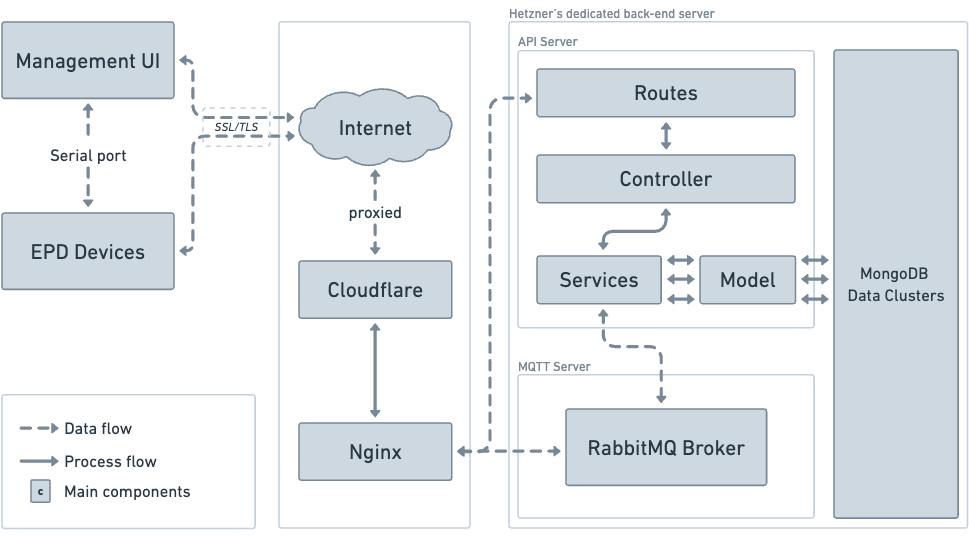
\includegraphics[scale=0.46]{doc/imgs/overall-architecture.png}
    \caption{Overall architecture of the system}
    \label{fig:Fig1}
\end{figure}

Figure \ref{fig:Fig1} illustrates the system's general architecture and provides an overview of its data flow. The system strategically uses the combination of MVCS (Model-View-Controller-Service) and microservice architectures to take advantage of their unique strengths in specific aspects. This hybrid architecture leverages the benefits of both architectural styles, such as scalability, flexibility, and the ability to use different technologies and patterns within each service.

Microservices architecture is a software development method that structures an application as a collection of loosely coupled services. In this architecture, each service can be developed, deployed, and scaled independently, allowing greater scalability, flexibility, and agility than monolithic architectures, as teams can update or fix individual components without impacting the entire system in case of failure. Thanks to its ability to accommodate the dynamic and distributed natures of IoT applications, microservice architecture is frequently used in various IoT projects. It allows organizations to build more agile and adaptive applications to handle the complex demands of modern business environments.

On the other hand, the Model-View-Controller-Service (MVCS) architecture is an extension of the traditional Model-View-Controller (MVC) pattern. It introduces a service layer sitting between the Controller and the Model, responsible for containing business logic and rules. This layer abstracts complex business operations, allowing Controllers to focus on handling incoming requests and delegating the heavy lifting to Services. This design pattern is well-suited to many web applications, providing a structured and organized approach to developing complex applications and making it easier to manage, maintain, and scale the system over time.

By combining these two architectures, the system is better equipped to handle the dynamic and distributed nature of IoT applications. It also enables organizations to build more agile and adaptive applications to address the complex demands of modern business environments while ensuring scalability, reliability, and seamless communication between different components.

\subsection{Overall design}
The system is divided into independently deployable services, including the API back-end server and MQTT Server. These services communicate via the MQTT protocol, and the MQTT Server also acts as a broker to relay data to the \gls{EPD} devices (Figure \ref{fig:Fig3}). API server follows the MVCS pattern with three main components: Controllers handling incoming requests and coordinating responses, Services containing the business logic and rules of the application, and Models interacting with the database, managing data storage and retrieval, while Management UI and \gls{EPD} devices act as a View component (Figure \ref{fig:Fig2}).
\subsubsection{MVCS architecture}
The system has three data types, and the packages of each type handling operation share the same structure: the Controller handles requests about the data type and delegates them to the Service, which processes the requests and uses the Model to interact with the database.
\begin{figure}[H]
    \centering
    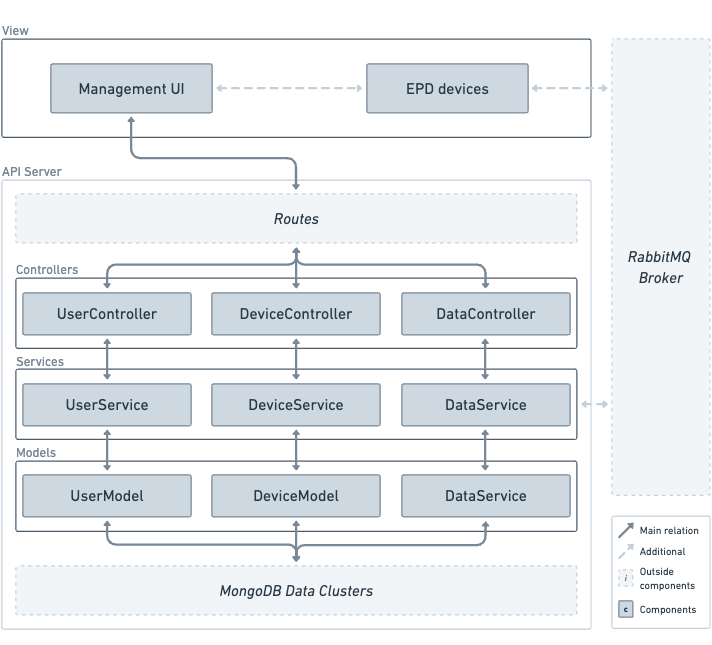
\includegraphics[scale=0.6]{doc/imgs/api-server.png}
    \caption{MVCS architecture}
    \label{fig:Fig2}
\end{figure}

\subsubsection{MQTT Service}
This service in the system acts as an intermediary, managing the state of all MQTT client connections, subscriptions, and message exchanges.
\begin{figure}[H]
    \centering
    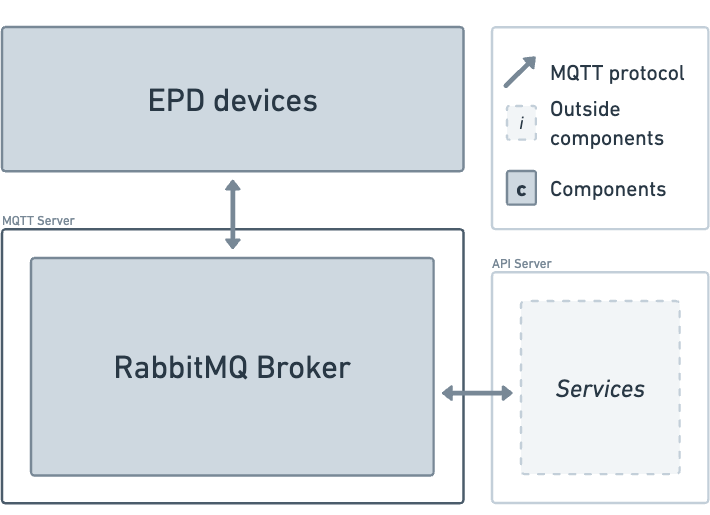
\includegraphics[scale=0.3]{doc/imgs/mqtt-server.png}
    \caption{MQTT microservice}
    \label{fig:Fig3}
\end{figure}

\subsection{Detailed package design}
\subsubsection{Models}
\begin{figure}[H]
    \centering
    \begin{tikzpicture}[]
         \begin{umlpackage}[fill = white]{Models}
            \umlclass[x = 2, y = 6, scale = 0.5, fill = white]{UserModel}{
                email: string \\
                password: string \\
                name: string \\
                gender: string \\
                \_id: ObjectId \\
                createdAt: time \\
                updatedAt: time
            }{
                \umlvirt{UserModel(userModel: dict): UserModel} \\
                findByIdAndUpdate(id: string): UserModel \\
                findById(id: string): UserModel \\
                findByIdAndRemove(id: string): void \\
                create(data: dict): UserModel \\
                findOne(filter: dict): UserModel
            }

            \umlclass[x = 0, y = 0, scale = 0.5, fill = white]{DeviceModel}{
                \_id: ObjectId \\
                name: string \\
                ssid: string \\
                pass: string \\
                dataID: ObjectId \\
                dataName: string \\
                active: boolean \\
                createdBy: ObjectId \\
            }{
                \umlvirt{DeviceModel(deviceModel: dict): DeviceModel} \\
                findByIdAndUpdate(id: string): DeviceModel \\
                findById(id: string): DeviceModel \\
                findByIdAndRemove(id: string): void \\
                create(data: dict): DeviceModel \\
                findOne(filter: dict): DeviceModel \\
                find(filter: dict): Array(DeviceModel)
            }
            
            \umlclass[x = 7, y = 0, scale = 0.5, fill = white]{DataModel}{
                \_id: ObjectId \\
                type: string \\
                name: string \\
                email: string \\
                input2: string \\
                input3: string \\
                input4: string \\
                active: boolean \\
                activeStartTime: uint \\
                deviceID: ObjectId \\
                deviceName: string \\
                activeTimestamp: Array \\
                fontStyle: string \\
                designSchema: string \\
                createdBy: ObjectId
            }{
                \umlvirt{DataModel(deviceModel: dict): DataModel} \\
                findByIdAndUpdate(id: string): DataModel \\
                findById(id: string): DataModel \\
                findByIdAndRemove(id: string): void \\
                findByIdAndDelete(id: string): void \\
                create(data: dict): DataModel \\
                findOne(filter: dict): DataModel
            }
            
            \umlassoc[mult1=1, mult2=*, pos1=0.03, pos2=0.7, align1=left, align2=left]{UserModel}{DeviceModel}
            \umlassoc[mult1=1, mult2=*, pos1=0.03, pos2=0.9, align1=right, align2=right]{UserModel}{DataModel}

            % Bidirectional Dependency
            \umldashedline{DeviceModel}{DataModel}
            \umldep[arg=updates, pos=0.5]{DeviceModel}{DataModel}
            \umldep[pos=0.5]{DataModel}{DeviceModel}
         \end{umlpackage}
    \end{tikzpicture}
    \caption{Model class diagram}
    \label{fig:ModelClassDiagram}
\end{figure}

\subsubsection{Services}
\begin{figure}[H]
    \centering
    \begin{tikzpicture}[]
         \begin{umlpackage}[fill = white]{Services}
            \umlclass[x = 1, y = 2.5, scale = 0.5, fill = white]{UserService}{}{
                findUserByEmail(email: string): UserModel \\
                createUser(user: dict): UserModel \\
                getUserById(id: string): UserModel \\
                updateUser(id: string, user: dict): UserModel \\
            }

            \umlclass[x = 0, y = 0, scale = 0.5, fill = white]{DeviceService}{}{
                getAllDevices(filter: dict): Array(DeviceModel) \\
                getDeviceById(id: string): DeviceModel \\
                createDevice(data: dict, userId: string): DeviceModel \\
                updateDevice(id: string, data: dict): DeviceModel \\
                deleteDevice(id: string, userId: string): void
            }
            
            \umlclass[x = 6, y = 0, scale = 0.5, fill = white]{DataService}{}{
                findDataByEmail(email: string): DataModel \\
                getAllData(filter: dict): Array(DataModel) \\
                getDataById(id: string): DataModel \\
                createData(data: dict, userId: string): DataModel \\
                updateData(id: string, data: dict): DataModel \\
                deleteData(id: string, userId: string): void
            }
         \end{umlpackage}
    \end{tikzpicture}
    \caption{Service class diagram}
    \label{fig:ServiceClassDiagram}
\end{figure}

\subsubsection{Controllers}
\begin{figure}[H]
    \centering
    \begin{tikzpicture}[]
         \begin{umlpackage}[fill = white]{Controllers}
            \umlclass[x = 3, y = 3, scale = 0.5, fill = white]{UserController}{
                userService: UserService
            }{
                register(): void \\
                login(id: string): void \\
                getAccountById(): UserModel \\
                updateAccount(): UserModel
            }

            \umlclass[x = 0, y = 0, scale = 0.5, fill = white]{DeviceController}{
                deviceService: DeviceService
            }{
                
                getAllDevices(): Array(DeviceModel) \\
                createDevice(): DeviceModel \\
                getDeviceById(): DeviceModel \\
                updateDevice(): DeviceModel \\
                deleteDevice(): void
            }
            
            \umlclass[x = 5, y = 0, scale = 0.5, fill = white]{DataController}{
                dataService: DataService
            }{
                getAllData(): Array(DataModel) \\
                createData(): DataModel \\
                getDataById(): DataModel \\
                updateData(): DataModel \\
                deleteData(): void
            }
            
         \end{umlpackage}
    \end{tikzpicture}
    \caption{Controller Class diagram}
    \label{fig:DataClassDiagram}
\end{figure}

\subsubsection{Views}
\begin{figure}[H]
    \centering
    \begin{tikzpicture}[]
         \begin{umlpackage}[fill = white]{Views}
            \umlclass[x = -1, y = 3, scale = 0.5, fill = white]{AccountView}{}{
                handleSubmit(e: event): void \\
            }
            
            \umlclass[x = 2.6, y = 3, scale = 0.5, fill = white]{NewDeviceView}{}{
                connectESP(): void \\
                handleSubmit(e: event): void \\
                handleReset(): void
            }

            \umlclass[x = 6.2, y = 3, scale = 0.5, fill = white]{DeviceView}{}{
                connectESP(): void \\
                deleteItem(): void \\
                handleSubmit(e: event): void \\
                handleReset(): void
            }
            
            \umlclass[x = 0, y = 1, scale = 0.5, fill = white]{NewDataView}{}{
                handleStage(e: event): void \\
                handleSubmit(e: event): void \\
                handleReset(): void \\
                getActiveDevices(): Array(DeviceModel)
            }

            \umlclass[x = 5, y = 1, scale = 0.5, fill = white]{DataView}{}{
                handleSubmit(e: event): void \\
                deleteItem(): void \\
                getActiveDevices(): Array(DeviceModel)
            }
         \end{umlpackage}
    \end{tikzpicture}
    \caption{View Class diagram}
    \label{fig:DataClassDiagram}
\end{figure}


\section{Detailed design}
\subsection{User interface design}
This system's architecture and user interface are meticulously tailored for computer displays, ensuring optimal functionality and visual experience on larger screens. The design is customized to leverage the expansive real estate of computer monitors (ranging from 1366 \(\times\) 768 and higher), facilitating ease of use and comprehensive information display. This focus on computer-targeted design means that the system is not intended for mobile use. As such, it may not provide an ideal user experience or full functionality on smaller mobile device screens. The decision to specialize in computer displays stems from a commitment to delivering a high-quality, immersive experience that fully utilizes the capabilities and advantages of larger screens typically associated with desktop or laptop computers.

There are four main layouts used on the website: authentication, dashboard, modal, and creation. The users use the authentication page (figure \ref{fig:Mockup1}) for authenticating purposes, including sign-in and sign-up. The dashboard page layout in picture \ref{fig:Mockup2} shows a table of \gls{EPD} devices and data, listing all information about each item and the buttons on the right side to open functional modals to view, edit, and delete, which are illustrated in figure \ref{fig:Mockup3}. In the creation page in figure \ref{fig:Mockup4}, users can create new devices and data by providing details in the inputs and choosing options from the dropdown. The layouts and the buttons follow the minimalistic design pattern and colors, improving the visual experience for users.

\begin{figure}[H]
    \centering
    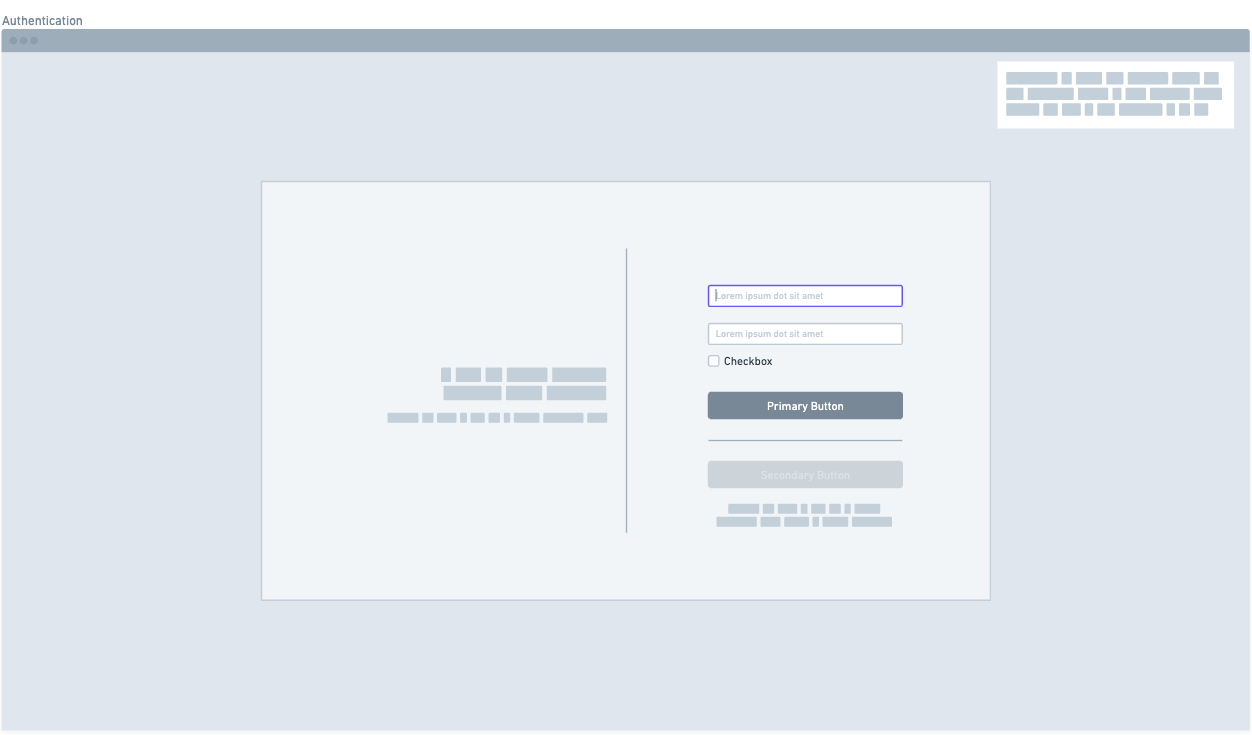
\includegraphics[scale=0.3]{doc/imgs/mockup1.png}
    \caption{Mockup display of authentication page}
    \label{fig:Mockup1}
\end{figure}
\begin{figure}[H]
    \centering
    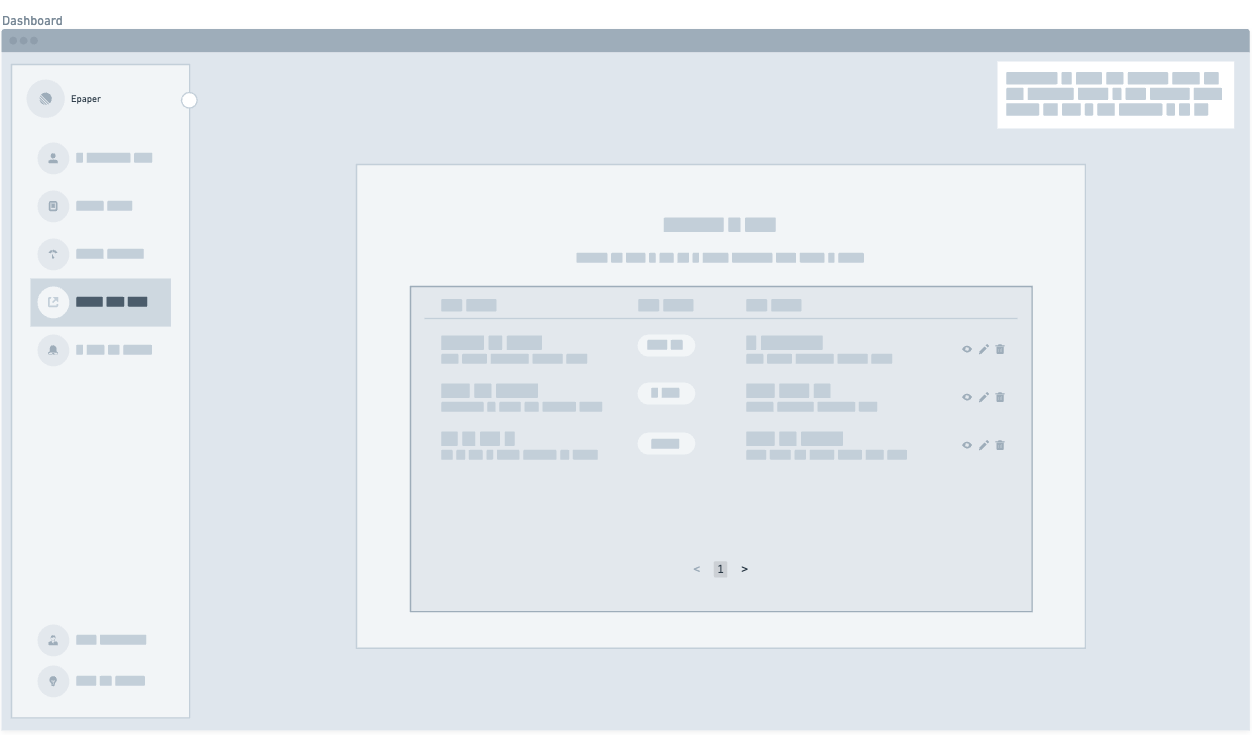
\includegraphics[scale=0.3]{doc/imgs/mockup2.png}
    \caption{Mockup display of dashboard page}
    \label{fig:Mockup2}
\end{figure}
\begin{figure}[H]
    \centering
    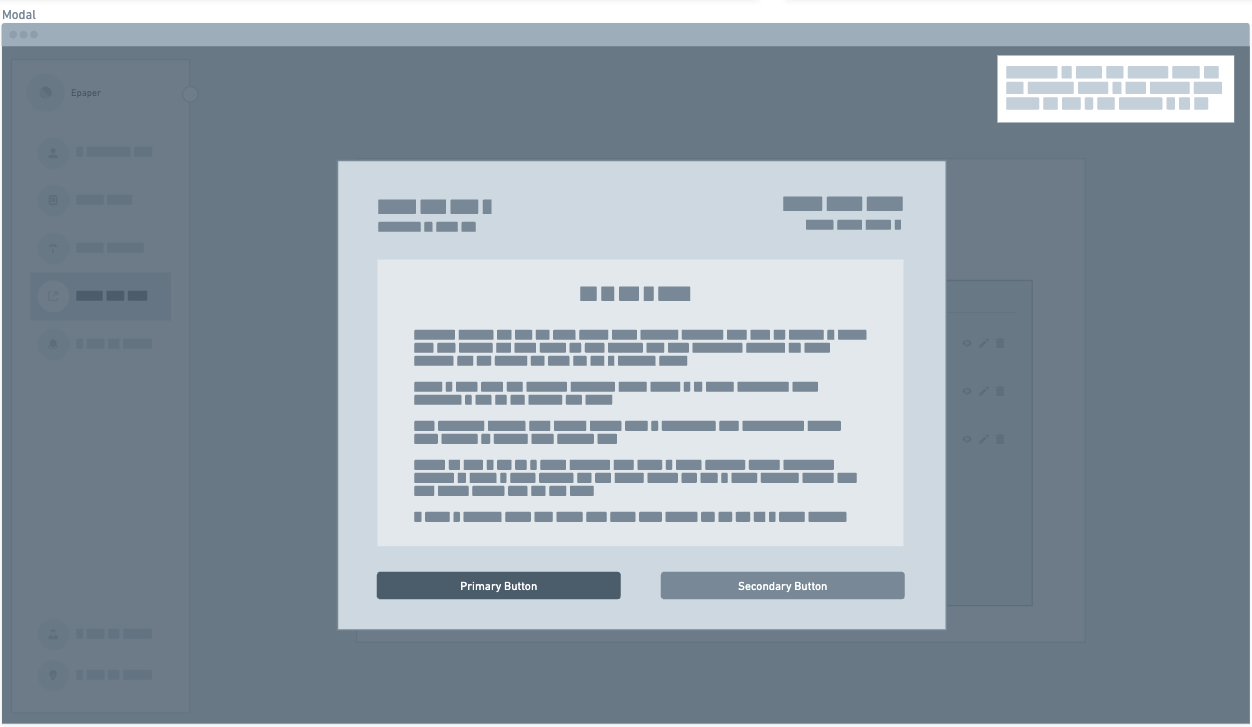
\includegraphics[scale=0.3]{doc/imgs/mockup3.png}
    \caption{Mockup display of modal component}
    \label{fig:Mockup3}
\end{figure}
\begin{figure}[H]
    \centering
    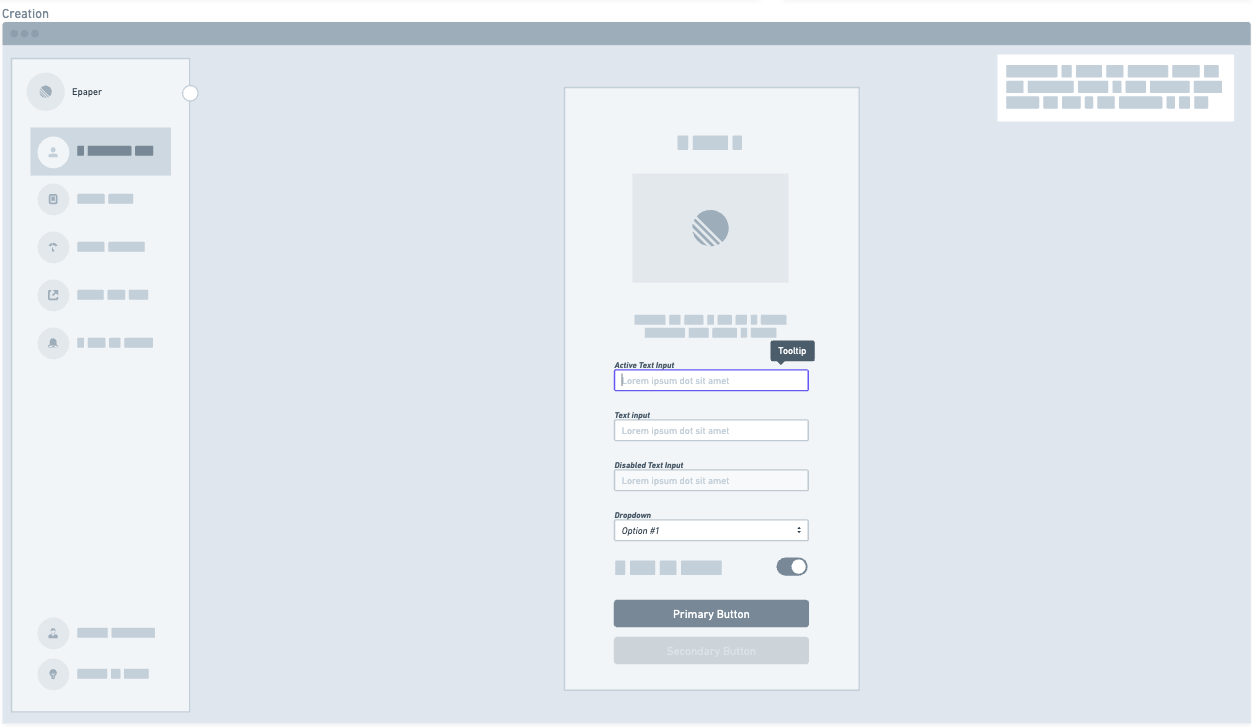
\includegraphics[scale=0.3]{doc/imgs/mockup4.png}
    \caption{Mockup display of creation page}
    \label{fig:Mockup4}
\end{figure}

\subsection{Layer design}
Each sub-section below demonstrates the workflow of each class participating in each use case in the form of a class diagram and a responding sequence diagram. Each class only shows relevant methods used in the use case.

\subsubsection{Class and sequence diagram of use case "Register a new device"}
\begin{figure}[H]
    \centering
    \begin{tikzpicture}
        % \draw (-1.5, 2.5) rectangle (13, -8);
    
        % Define system boundary
        \umlactor[x = -0.5, y = 4, scale = 0.7]{Manager}
        \umlactor[x = 2, y = 4.5, scale = 0.7]{EPD Devices}
        
        \begin{umlpackage}[fill = white]{pkg}
            \umlclass[x = 0, y = 7, scale = 0.5, fill = white]{NewDeviceView}{}{
                connectESP(): void \\
                handleSubmit(e: event): void \\
                handleReset(): void
            }
            
            \umlclass[x = 4, y = 7, scale = 0.5, fill = white]{DeviceController}{
                deviceService: DeviceService
            }{
                createDevice(): DeviceModel
            }

            \umlclass[x = 3, y = 2, scale = 0.5, fill = white]{DeviceService}{}{
                createDevice(data: dict, userId: string): DeviceModel
            }

            \umlclass[x = 6, y = 4.5, scale = 0.5, fill = white]{DeviceModel}{
                \_id: ObjectId \\
                name: string \\
                ssid: string \\
                pass: string \\
                dataID: ObjectId \\
                dataName: string \\
                active: boolean \\
                createdBy: ObjectId \\
            }{
                create(data: dict): DeviceModel
            }
        \end{umlpackage}
        
        \umluniassoc[]{Manager}{NewDeviceView}
        \umluniassoc[]{NewDeviceView}{EPD Devices}
        \umluniassoc[]{NewDeviceView}{DeviceController}
        \umluniassoc[]{DeviceController}{DeviceService}
        \umluniassoc[]{DeviceService}{DeviceModel}
    \end{tikzpicture}
    \caption{Class diagram of use case "Register a new device"}
    \label{fig:usecasediagram}
\end{figure}

\begin{figure}[H]
    \centering
    \begin{tikzpicture}[every node/.style={scale=0.8, font=\tiny}]
        \begin{umlseqdiag}
            \umlactor[no ddots, scale = 1.6, x = -1]{Manager}
            \umlactor[no ddots, scale = 1.6, x = 0.5]{EPD Device}
            \umlboundary[no ddots, scale = 1.6, x = 2.7]{NewDeviceView}
            \umlcontrol[no ddots, scale = 1.6, x = 5.2]{DeviceController}
            \umlcontrol[no ddots, scale = 1.6, x = 7.7]{DeviceService}
            \umlentity[no ddots, scale = 1.6, x = 10]{DeviceModel}
            \umlentity[no ddots, scale = 1.6, x = 12]{MQTT Broker}

            \begin{umlcall}[op={Connect ESP device}, dt = 5]{Manager}{NewDeviceView}
                \begin{umlcall}[op={connectESP()}, dt = 5, with return]{NewDeviceView}{EPD Device}
                \end{umlcall}
            \end{umlcall}
            
            \begin{umlcall}[op={handleSubmit()}, with return]{Manager}{NewDeviceView}
                \begin{umlcall}[op={createDevice()}, return = {device}]{NewDeviceView}{DeviceController}
                    \begin{umlcall}[op={createDevice()}, return = {device}]{DeviceController}{DeviceService}
                        \begin{umlcall}[op={create()}, return = {device}]{DeviceService}{DeviceModel}
                        \end{umlcall}
                        \begin{umlcall}[op={subscribe()}, return = {acknowledge}]{DeviceService}{MQTT Broker}
                        \end{umlcall}
                    \end{umlcall}
                \end{umlcall}
                
                \begin{umlcall}[op={write()}, with return]{NewDeviceView}{EPD Device}
                    \begin{umlcall}[op={subscribe()}, return = {acknowledge}]{EPD Device}{MQTT Broker}
                    \end{umlcall}
                \end{umlcall}
            \end{umlcall}
                
        \end{umlseqdiag}
    \end{tikzpicture}
    \caption{Sequence diagram of use case "Register a new device"}
    \label{fig:enter-label}
\end{figure}


\subsubsection{Class and sequence diagram of use case "Add a new data"}
\begin{figure}[H]
    \centering
    \begin{tikzpicture}
        % Define system boundary
        \umlactor[x = 3, y = 10, scale = 0.7]{Manager}
        \umlactor[x = 9.5, y = 4, scale = 0.7]{EPD Devices}
        
        \begin{umlpackage}[fill = white]{pkg}
            \umlclass[x = 8, y = 10, scale = 0.5, fill = white]{NewDataView}{}{
                handleStage(e: event): void \\
                handleSubmit(e: event): void \\
                handleReset(): void \\
                getActiveDevices(): Array(DeviceModel)
            }

            \umlclass[x = 3, y = 7.5, scale = 0.5, fill = white]{DataController}{
                dataService: DataService
            }{
                createData(): DataModel
            }

            \umlclass[x = 8, y = 7.5, scale = 0.5, fill = white]{DeviceController}{
                deviceService: DeviceService
            }{
                getAllDevices(): Array(DeviceModel) \\
                updateDevice(): DeviceModel
            }

            \umlclass[x = 5, y = 5, scale = 0.5, fill = white]{DataService}{}{
                createData(data: dict, userId: string): DataModel
            }

            \umlclass[x = 4, y = 2, scale = 0.5, fill = white]{DeviceService}{}{
                getAllDevices(filter: dict): Array(DeviceModel)
            }

            \umlclass[x = 14, y = 2, scale = 0.5, fill = white]{DeviceModel}{
                \_id: ObjectId \\
                name: string \\
                ssid: string \\
                pass: string \\
                dataID: ObjectId \\
                dataName: string \\
                active: boolean \\
                createdBy: ObjectId \\
            }{
                findByIdAndUpdate(id: string): DeviceModel \\
                findById(id: string): DeviceModel \\
                find(filter: dict): Array(DeviceModel)
            }
            
            \umlclass[x = 13, y = 8, scale = 0.5, fill = white]{DataModel}{
                \_id: ObjectId \\
                type: string \\
                name: string \\
                email: string \\
                input2: string \\
                input3: string \\
                input4: string \\
                active: boolean \\
                activeStartTime: uint \\
                deviceID: ObjectId \\
                deviceName: string \\
                activeTimestamp: Array \\
                fontStyle: string \\
                designSchema: string \\
                createdBy: ObjectId
            }{
                findByIdAndUpdate(id: string): DataModel \\
                findById(id: string): DataModel \\
                create(data: dict): DataModel
            }
        \end{umlpackage}
        
        \umluniassoc[]{Manager}{NewDataView}
        \umluniassoc[geometry = |-, anchor1 = 80, anchor2 = -180]{DataService}{EPD Devices}
        \umluniassoc[geometry = |-, anchor1 = 100, anchor2 = -180]{DeviceService}{EPD Devices}
        \umluniassoc[]{NewDataView}{DataController}
        \umluniassoc[]{NewDataView}{DeviceController}
        \umluniassoc[]{DataController}{DataService}
        \umluniassoc[geometry = |-, anchor1 = -90, anchor2 = 5]{DeviceController}{DeviceService}
        \umluniassoc[geometry = -|, anchor1 = 0, anchor2 = -90]{DataService}{DataModel}
        \umluniassoc[geometry = -|, anchor1 = 0, anchor2 = 90]{DataService}{DeviceModel}
        \umluniassoc[]{DeviceService}{DeviceModel}
    \end{tikzpicture}
    \caption{Class diagram of use case "Add a new data"}
    \label{fig:usecasediagram}
\end{figure}

\begin{landscape}
    \begin{figure}[H]
        \centering
        \begin{tikzpicture}[every node/.style={font=\tiny}]
            \begin{umlseqdiag}
                \umlactor[no ddots, scale = 1, x = -2]{Manager}
                \umlactor[no ddots, scale = 1, x = 0.3, y = -5]{EPD Device}
                \umlboundary[no ddots, scale = 1, x = 2.5]{NewDataView}
                \umlcontrol[no ddots, scale = 1, x = 4.5, y = -2]{DataController}
                \umlcontrol[no ddots, scale = 1, x = 7]{DeviceController}
                \umlcontrol[no ddots, scale = 1, x = 9, y = -2]{DataService}
                \umlcontrol[no ddots, scale = 1, x = 11.5]{DeviceService}
                \umlentity[no ddots, scale = 1, x = 14, y = -2]{DataModel}
                \umlentity[no ddots, scale = 1, x = 16.5]{DeviceModel}

                % \umlsdnode[dt=60]{EPD Device}
                \umlsdnode[dt=49]{DataController}
                \umlsdnode[dt=49]{DataService}
                \umlsdnode[dt=49]{DataModel}

                \begin{umlcall}[op={Select data type}, dt = 4, with return]{Manager}{NewDataView}\end{umlcall}
                \begin{umlcall}[op={Fill submit form}, dt = 3, with return]{Manager}{NewDataView}\end{umlcall}
                
                \begin{umlfragment}[type=alt, label={display.true}, inner xsep = 9]
                    \begin{umlcall}[op={getAllDevices(fitlers)}, dt = 6, return = {devices}]{Manager}{NewDataView}
                        \begin{umlcall}[op={getAllDevices(filters)}, dt = 1, return={devices}]{NewDataView}{DeviceController}
                            \begin{umlcall}[op={getAllDevices(filters)}, dt = 1, return={devices}]{DeviceController}{DeviceService}
                                \begin{umlcall}[op={find()}, dt = 1, return={devices}]{DeviceService}{DeviceModel}\end{umlcall}
                                
                                \begin{umlfragment}[type=loop, inner xsep = 2]
                                    \begin{umlcall}[op={ping()}, dt = 3, return = {pingOK}]{DeviceService}{EPD Device}\end{umlcall}
                                    \begin{umlcall}[op={findById()}, dt = 1, return = {device}]{DeviceService}{DeviceModel}\end{umlcall}
                                    \begin{umlcall}[op={findByIdAndUpdate()}, dt = 3]{DeviceService}{DeviceModel}\end{umlcall}
                                \end{umlfragment}
                                
                                \begin{umlcall}[op={find()}, dt = 2, return={devices}]{DeviceService}{DeviceModel}
                                \end{umlcall}
                            \end{umlcall}
                        \end{umlcall}
                    \end{umlcall}
                \end{umlfragment}
                    
            \end{umlseqdiag}
        \end{tikzpicture}
        \caption{Sequence diagram of use case "Add a new data" | Cont’d on next page}
        \label{fig:enter-label}
    \end{figure}
\end{landscape}

\begin{landscape}
    \begin{figure}[H]
        \centering
        \begin{tikzpicture}[every node/.style={font=\tiny}]
            \begin{umlseqdiag}
                \umlactor[no ddots, scale = 1, x = -2]{Manager}
                \umlactor[no ddots, scale = 1, x = 0.3, y = -6]{EPD Device}
                \umlboundary[no ddots, scale = 1, x = 2]{NewDataView}
                \umlcontrol[no ddots, scale = 1, x = 5.5]{DataController}
                \umlcontrol[no ddots, scale = 1, x = 8, y = -0.5]{DeviceController}
                \umlcontrol[no ddots, scale = 1, x = 10]{DataService}
                \umlcontrol[no ddots, scale = 1, x = 12.5, y = -0.6]{DeviceService}
                \umlentity[no ddots, scale = 1, x = 15]{DataModel}
                \umlentity[no ddots, scale = 1, x = 17, y = -1.2]{DeviceModel}
                
                \umlsdnode[dt=57]{DeviceController}
                \umlsdnode[dt=53]{DeviceService}
            
                \begin{umlcall}[op={handleSubmit()}, with return, dt=4]{Manager}{NewDataView}
                    \begin{umlcall}[op={createData()}, dt = 1, return = {data}]{NewDataView}{DataController}
                        \begin{umlcall}[op={createData()}, dt = 1, return = {data}]{DataController}{DataService}
                            \begin{umlcall}[op={create()}, dt = 1, return = {data}]{DataService}{DataModel}\end{umlcall}
                            
                            \begin{umlfragment}[type=alt, label={data.active}, inner xsep = 9]
                                \begin{umlcall}[op={publish()}, dt=3, return = {writeOK}]{DataService}{EPD Device}\end{umlcall}
                                \begin{umlcall}[op={findById()}, dt=1, return = {device}]{DataService}{DeviceModel}\end{umlcall}
                                
                                \begin{umlfragment}[type=alt, label={old data?}, inner xsep = 7]
                                    \begin{umlcall}[op={findById()}, dt=2, return = {oldData}]{DataService}{DataModel}\end{umlcall}
                                    \begin{umlcall}[op={findByIdAndUpdate()}]{DataService}{DataModel}\end{umlcall}
                                \end{umlfragment}

                                \begin{umlcall}[op={findByIdAndUpdate()}, dt=2]{DataService}{DataModel}\end{umlcall}
                                \begin{umlcall}[op={findByIdAndUpdate()}, dt=4]{DataService}{DeviceModel}\end{umlcall}
                                \begin{umlcall}[op={findById()}, return = {data}]{DataService}{DeviceModel}\end{umlcall}
                            \end{umlfragment}
                        \end{umlcall}
                    \end{umlcall}
                \end{umlcall}
                
            \end{umlseqdiag}
        \end{tikzpicture}
        \caption{cont’d from previous page}
        \label{fig:enter-label}
    \end{figure}
\end{landscape}




\subsubsection{Class and sequence diagram of use case "Change a device information"}
\begin{figure}[H]
    \centering
    \begin{tikzpicture}
        % Define system boundary
        \umlactor[x = 3, y = 10, scale = 0.7]{Manager}
        \umlactor[x = 3, y = 7, scale = 0.7]{EPD Devices}

        \begin{umlpackage}[fill = white]{pkg}
            \umlclass[x = 7, y = 10, scale = 0.5, fill = white]{DeviceView}{}{
                connectESP(): void \\
                handleSubmit(e: event): void \\
                handleReset(): void
            }

            \umlclass[x = 7, y = 7, scale = 0.5, fill = white]{DeviceController}{
                deviceService: DeviceService
            }{
                getDeviceById(): DeviceModel \\
                updateDevice(): DeviceModel
            }

            \umlclass[x = 9, y = 4, scale = 0.5, fill = white]{DeviceService}{}{
                getDeviceById(id: string): DeviceModel \\
                updateDevice(id: string, data: dict): DeviceModel
            }

            \umlclass[x = 3.5, y = 4, scale = 0.5, fill = white]{DeviceModel}{
                \_id: ObjectId \\
                name: string \\
                ssid: string \\
                pass: string \\
                dataID: ObjectId \\
                dataName: string \\
                active: boolean \\
                createdBy: ObjectId \\
            }{
                findById(id: string): DeviceModel \\
                findByIdAndUpdate(id: string): DeviceModel
            }
            
            \umlclass[x = 11, y = 8, scale = 0.5, fill = white]{DataModel}{
                \_id: ObjectId \\
                type: string \\
                name: string \\
                email: string \\
                input2: string \\
                input3: string \\
                input4: string \\
                active: boolean \\
                activeStartTime: uint \\
                deviceID: ObjectId \\
                deviceName: string \\
                activeTimestamp: Array \\
                fontStyle: string \\
                designSchema: string \\
                createdBy: ObjectId
            }{
                findByIdAndUpdate(id: string): DataModel \\
                findById(id: string): DataModel
            }
        \end{umlpackage}
        
        \umluniassoc[]{Manager}{DeviceView}
        \umluniassoc[]{DeviceService}{EPD Devices}
        \umluniassoc[]{DeviceView}{EPD Devices}
        \umluniassoc[]{DeviceView}{DeviceController}
        \umluniassoc[]{DeviceController}{DeviceService}
        \umluniassoc[]{DeviceService}{DataModel}
        \umluniassoc[]{DeviceService}{DeviceModel}
    \end{tikzpicture}
    \caption{Class diagram of use case "Change a device information"}
    \label{fig:usecasediagram}
\end{figure}

\begin{landscape}
    \begin{figure}[h]
        \centering
        \begin{tikzpicture}[every node/.style={font=\tiny}]
            \begin{umlseqdiag}
                \umlactor[no ddots, x = -4]{Manager}
                \umlactor[no ddots, x = -1.5]{EPD Device}
                \umlboundary[no ddots, x = 2]{DeviceView}
                \umlcontrol[no ddots, x = 6]{DeviceController}
                \umlcontrol[no ddots, x = 10]{DeviceService}
                \umlentity[no ddots, x = 15]{DeviceModel}
                \umlentity[no ddots, x = 18]{DataModel}
    
                \begin{umlfragment}[type=alt, label={not active}, inner xsep = 8]
                    \begin{umlcall}[op={ConnectESP()}, dt=6]{Manager}{DeviceView} 
                        \begin{umlcall}[op={ConnectESP()}, dt=3.5, with return]{DeviceView}{EPD Device}\end{umlcall}
                    \end{umlcall}
                \end{umlfragment}
                    
                \begin{umlcall}[op={handleSubmit()}, dt = 5, with return]{Manager}{DeviceView} 
                    \begin{umlcall}[op={updateDevice()}, dt=2, return={device}]{DeviceView}{DeviceController} 
                        \begin{umlcall}[op={updateDevice()}, dt=2, return={device}]{DeviceController}{DeviceService}
                            \begin{umlcall}[op={publish()}, dt=4, return = {updateOK}]{DeviceService}{EPD Device}\end{umlcall}
                            
                            \begin{umlfragment}[type=alt, label={have data}, inner xsep = 9]
                                \begin{umlcall}[op={findById()}, dt=2, return={data}]{DeviceService}{DataModel}\end{umlcall}
                                \begin{umlcall}[op={findByIdAndUpdate()}, dt=5]{DeviceService}{DataModel}\end{umlcall}
                            \end{umlfragment}
                            
                            \begin{umlcall}[op={findByIdAndUpdate()}, dt=2, return={device}]{DeviceService}{DeviceModel}\end{umlcall}
                        \end{umlcall}
                    \end{umlcall}

                \begin{umlfragment}[type=alt, label={not active}, inner xsep = 8]
                    \begin{umlcall}[op={write()}, dt=2]{DeviceView}{EPD Device}\end{umlcall}
                \end{umlfragment}
                \end{umlcall}
            \end{umlseqdiag}
        \end{tikzpicture}
        \caption{Sequence diagram of use case "Change a device information"}
        \label{fig:enter-label}
    \end{figure}
\end{landscape}

\subsubsection{Class and sequence diagram of use case "Change data information"}
\begin{figure}[H]
    \centering
    \begin{tikzpicture}
        % Define system boundary
        \umlactor[x = 3, y = 10, scale = 0.7]{Manager}
        \umlactor[x = 9.5, y = 4, scale = 0.7]{EPD Devices}
        
        \begin{umlpackage}[fill = white]{pkg}
            \umlclass[x = 8, y = 10, scale = 0.5, fill = white, fill = white]{DataView}{}{
                handleSubmit(e: event): void \\
                getActiveDevices(): Array(DeviceModel)
            }

            \umlclass[x = 3, y = 7.5, scale = 0.5, fill = white]{DataController}{
                dataService: DataService
            }{
                getDataById(): DataModel \\
                updateData(): DataModel
            }

            \umlclass[x = 8, y = 7.5, scale = 0.5, fill = white]{DeviceController}{
                deviceService: DeviceService
            }{
                getAllDevices(): Array(DeviceModel) \\
                updateDevice(): DeviceModel
            }

            \umlclass[x = 5, y = 5, scale = 0.5, fill = white]{DataService}{}{
                getDataById(id: string): DataModel \\
                updateData(id: string, data: dict): DataModel
            }

            \umlclass[x = 4, y = 2, scale = 0.5, fill = white]{DeviceService}{}{
                getAllDevices(filter: dict): Array(DeviceModel)
            }

            \umlclass[x = 14, y = 2, scale = 0.5, fill = white]{DeviceModel}{
                \_id: ObjectId \\
                name: string \\
                ssid: string \\
                pass: string \\
                dataID: ObjectId \\
                dataName: string \\
                active: boolean \\
                createdBy: ObjectId \\
            }{
                findByIdAndUpdate(id: string): DeviceModel \\
                findById(id: string): DeviceModel \\
                find(filter: dict): Array(DeviceModel)
            }
            
            \umlclass[x = 13, y = 8, scale = 0.5, fill = white]{DataModel}{
                \_id: ObjectId \\
                type: string \\
                name: string \\
                email: string \\
                input2: string \\
                input3: string \\
                input4: string \\
                active: boolean \\
                activeStartTime: uint \\
                deviceID: ObjectId \\
                deviceName: string \\
                activeTimestamp: Array \\
                fontStyle: string \\
                designSchema: string \\
                createdBy: ObjectId
            }{
                findByIdAndUpdate(id: string): DataModel \\
                findById(id: string): DataModel \\
            }
        \end{umlpackage}
        
        \umluniassoc[]{Manager}{DataView}
        \umluniassoc[geometry = |-, anchor1 = 80, anchor2 = -180]{DataService}{EPD Devices}
        \umluniassoc[geometry = |-, anchor1 = 100, anchor2 = -180]{DeviceService}{EPD Devices}
        \umluniassoc[]{DataView}{DataController}
        \umluniassoc[]{DataView}{DeviceController}
        \umluniassoc[]{DataController}{DataService}
        \umluniassoc[geometry = |-, anchor1 = -90, anchor2 = 5]{DeviceController}{DeviceService}
        \umluniassoc[geometry = -|, anchor1 = 0, anchor2 = -90]{DataService}{DataModel}
        \umluniassoc[geometry = -|, anchor1 = 0, anchor2 = 90]{DataService}{DeviceModel}
        \umluniassoc[]{DeviceService}{DeviceModel}
    \end{tikzpicture}
    \caption{Class diagram of use case "Change data information"}
    \label{fig:usecasediagram}
\end{figure}

\begin{landscape}
    \begin{figure}[H]
        \centering
        \begin{tikzpicture}[every node/.style={font=\tiny}]
            \begin{umlseqdiag}
                \umlactor[no ddots, scale = 1, x = -2]{Manager}
                \umlactor[no ddots, scale = 1, x = 0.3, y = -4]{EPD Device}
                \umlboundary[no ddots, scale = 1, x = 2.5]{DataView}
                \umlcontrol[no ddots, scale = 1, x = 4.5, y = -1]{DataController}
                \umlcontrol[no ddots, scale = 1, x = 7]{DeviceController}
                \umlcontrol[no ddots, scale = 1, x = 9, y = -1]{DataService}
                \umlcontrol[no ddots, scale = 1, x = 11.5]{DeviceService}
                \umlentity[no ddots, scale = 1, x = 14, y = -1]{DataModel}
                \umlentity[no ddots, scale = 1, x = 16.5]{DeviceModel}

                \umlsdnode[dt=50]{DataController}
                \umlsdnode[dt=50]{DataService}
                \umlsdnode[dt=50]{DataModel}

                \begin{umlcall}[op={Fill submit form}, dt = 4, with return]{Manager}{DataView}\end{umlcall}
                
                \begin{umlfragment}[type=alt, label={display.true}, inner xsep = 9]
                    \begin{umlcall}[op={getAllDevices(fitlers)}, dt = 7, return = {devices}]{Manager}{DataView}
                        \begin{umlcall}[op={getAllDevices(filters)}, dt = 2, return={devices}]{DataView}{DeviceController}
                            \begin{umlcall}[op={getAllDevices(filters)}, dt = 2, return={devices}]{DeviceController}{DeviceService}
                                \begin{umlcall}[op={find()}, dt = 2, return={devices}]{DeviceService}{DeviceModel}\end{umlcall}
                                
                                \begin{umlfragment}[type=loop, inner xsep = 2]
                                    \begin{umlcall}[op={ping()}, dt = 3, return = {pingOK}]{DeviceService}{EPD Device}\end{umlcall}
                                    \begin{umlcall}[op={findById()}, dt = 2, return = {device}]{DeviceService}{DeviceModel}\end{umlcall}
                                    \begin{umlcall}[op={findByIdAndUpdate()}, dt = 4]{DeviceService}{DeviceModel}\end{umlcall}
                                \end{umlfragment}
                                
                                \begin{umlcall}[op={find()}, dt = 2, return={devices}]{DeviceService}{DeviceModel}
                                \end{umlcall}
                            \end{umlcall}
                        \end{umlcall}
                    \end{umlcall}
                \end{umlfragment}
                    
            \end{umlseqdiag}
        \end{tikzpicture}
        \caption{Sequence diagram of use case "Change data information" | Cont’d on next page}
        \label{fig:enter-label}
    \end{figure}
\end{landscape}

\begin{landscape}
    \begin{figure}[H]
        \centering
        \begin{tikzpicture}[every node/.style={font=\small}]
            \begin{umlseqdiag}
                \umlactor[no ddots, scale = 0.7, x = -2]{Manager}
                \umlactor[no ddots, scale = 0.7, x = 0.3, y = -2.5]{EPD Device}
                \umlboundary[no ddots, scale = 0.7, x = 2]{DataView}
                \umlcontrol[no ddots, scale = 0.7, x = 5.5]{DataController}
                \umlcontrol[no ddots, scale = 0.7, x = 8, y = -0.7]{DeviceController}
                \umlcontrol[no ddots, scale = 0.7, x = 10]{DataService}
                \umlcontrol[no ddots, scale = 0.7, x = 12.5, y = -1.2]{DeviceService}
                \umlentity[no ddots, scale = 0.7, x = 15]{DataModel}
                \umlentity[no ddots, scale = 0.7, x = 17, y = -1.2]{DeviceModel}
                
                \begin{umlcall}[op={handleSubmit()}, with return, dt=4]{Manager}{DataView}
                    \begin{umlcall}[op={updateData()}, return = {data}]{DataView}{DataController}
                        \begin{umlcall}[op={updateData()}, dt = 2, return = {data}, padding=4]{DataController}{DataService}
                            \begin{umlcall}[op={findById()}, dt = 2, return = {oldData}]{DataService}{DataModel}\end{umlcall}
                            
                            \begin{umlfragment}[type=alt, label={oldData.active}, inner xsep = 10, inner ysep=0.3]
                                \begin{umlcall}[op={publish()}, dt = 4, return = {removeOK}]{DataService}{EPD Device}\end{umlcall}
                                \begin{umlcall}[op={findById()}, dt = 1, return = {device}]{DataService}{DeviceModel}\end{umlcall}
                                \begin{umlcall}[op={findByIdAndUpdate()}]{DataService}{DeviceModel}\end{umlcall}
                                
                                \begin{umlfragment}[type=alt, label={!data.active}, inner xsep = 6]
                                    \begin{umlcall}[op={findByIdAndUpdate()}, return = {data}, dt=0]{DataService}{DataModel}\end{umlcall}
                                \end{umlfragment}
                                
                                \umlfpart [default]
                                
                                \begin{umlfragment}[type=alt, name = alt, label={data.active}, inner xsep = 5, inner ysep = 0]
                                    \begin{umlcall}[dt = 4]{DataService}{DataService}\end{umlcall}
                                    % \begin{umlcall}[op={findById()}, return = {device}]{DataService}{DeviceModel}\end{umlcall}
                                    
                                    % \begin{umlfragment}[type=alt, label={old data?}, inner xsep = 7]
                                    %     \begin{umlcall}[op={findById()}, return = {oldData}]{DataService}{DataModel}\end{umlcall}
                                    %     \begin{umlcall}[op={findByIdAndUpdate()}]{DataService}{DataModel}\end{umlcall}
                                    % \end{umlfragment}
    
                                    % \begin{umlcall}[op={findByIdAndUpdate()}]{DataService}{DataModel}\end{umlcall}
                                    % \begin{umlcall}[op={findByIdAndUpdate()}]{DataService}{DeviceModel}\end{umlcall}
                                    % \begin{umlcall}[op={findById()}, return = {data}]{DataService}{DeviceModel}\end{umlcall}
                                \end{umlfragment}
                                \umlnote[x = 3, y = -8.5, fill = white]{alt}{This process of displaying on the device is the same as "Add a new data" process}
                                \begin{umlcall}[op={findByIdAndUpdate()}, dt = 4, return = {data}]{DataService}{DataModel}\end{umlcall}
                            \end{umlfragment}
                        \end{umlcall}
                    \end{umlcall}
                \end{umlcall}

            \end{umlseqdiag}
        \end{tikzpicture}
        \caption{cont’d from previous page}
        \label{fig:enter-label}
    \end{figure}
\end{landscape}

\subsubsection{Class and sequence diagram of use case "Remove a device"}
\begin{figure}[H]
    \centering
    \begin{tikzpicture}
        % Define system boundary
        \umlactor[x = 3, y = 10, scale = 0.7]{Manager}
        \umlactor[x = 3, y = 7, scale = 0.7]{EPD Devices}

        \begin{umlpackage}[fill = white]{pkg}
            \umlclass[x = 7, y = 10, scale = 0.5, fill = white]{DeviceView}{}{
                deleteItem(): void
            }

            \umlclass[x = 7, y = 7, scale = 0.5, fill = white]{DeviceController}{
                deviceService: DeviceService
            }{
                deleteDevice(): void
            }

            \umlclass[x = 9, y = 4, scale = 0.5, fill = white]{DeviceService}{}{
                getDeviceById(id: string): DeviceModel \\
                deleteDevice(id: string, userId: string): void
            }

            \umlclass[x = 3.5, y = 4, scale = 0.5, fill = white]{DeviceModel}{
                \_id: ObjectId \\
                name: string \\
                ssid: string \\
                pass: string \\
                dataID: ObjectId \\
                dataName: string \\
                active: boolean \\
                createdBy: ObjectId \\
            }{
                findByIdAndRemove(id: string): void \\
            }
            
            \umlclass[x = 11, y = 8, scale = 0.5, fill = white]{DataModel}{
                \_id: ObjectId \\
                type: string \\
                name: string \\
                email: string \\
                input2: string \\
                input3: string \\
                input4: string \\
                active: boolean \\
                activeStartTime: uint \\
                deviceID: ObjectId \\
                deviceName: string \\
                activeTimestamp: Array \\
                fontStyle: string \\
                designSchema: string \\
                createdBy: ObjectId
            }{
                findByIdAndUpdate(id: string): DataModel \\
            }
        \end{umlpackage}
        
        \umluniassoc[]{Manager}{DeviceView}
        \umluniassoc[]{DeviceService}{EPD Devices}
        \umluniassoc[]{DeviceView}{EPD Devices}
        \umluniassoc[]{DeviceView}{DeviceController}
        \umluniassoc[]{DeviceController}{DeviceService}
        \umluniassoc[]{DeviceService}{DataModel}
        \umluniassoc[]{DeviceService}{DeviceModel}
    \end{tikzpicture}
    \caption{Class diagram of use case "Remove a device"}
    \label{fig:usecasediagram}
\end{figure}

\begin{landscape}
    \begin{figure}[H]
        \centering
        \begin{tikzpicture}[every node/.style={font=\small}]
            \begin{umlseqdiag}
                \umlactor[no ddots, scale = 0.7, x = -4, y = -2]{EPD Device}
                \umlactor[no ddots, scale = 0.7, x = -1]{Manager}
                \umlboundary[no ddots, scale = 0.7, x = 2]{DeviceView}
                \umlcontrol[no ddots, scale = 0.7, x = 5.5]{DeviceController}
                \umlentity[no ddots, scale = 0.7, x = 8]{DataModel}
                \umlcontrol[no ddots, scale = 0.7, x = 12.7]{DeviceService}
                \umlentity[no ddots, scale = 0.7, x = 17]{DeviceModel}
     
                \begin{umlcall}[op={deleteItem()}, dt=3, return={success}]{Manager}{DeviceView} 
                    \begin{umlcall}[op={deleteDevice()}, dt=1, return={device}]{DeviceView}{DeviceController} 
                        \begin{umlcall}[op={deleteDevice()}, dt=1, return={device}]{DeviceController}{DeviceService}
                            \begin{umlcall}[op={findById()}, dt=1, return = {device}]{DeviceService}{DeviceModel} 
                            \end{umlcall}
                            
                            \begin{umlfragment}[type=alt, name = alt, inner ysep=-3]
                                \begin{umlcall}[op={null}, dt=13, padding=-11,type=return]{DeviceService}{DeviceController} 
                                    \begin{umlcall}[op={null}, dt=1, type=return]{DeviceController}{DeviceView}
                                        \begin{umlcall}[op={null}, dt=1, type=return]{DeviceView}{Manager}\end{umlcall}
                                    \end{umlcall}
                                \end{umlcall}
                            \end{umlfragment}
                            
                            \umlnote[x = 4, y = -7, fill = white]{alt}{(user incorrect and exist device) or not exist device}
                            
                            \begin{umlfragment}[type=alt, name = alt1]
                                \begin{umlcall}[op={publish()}, dt = 11, return = {removeOK}]{DeviceService}{EPD Device}\end{umlcall}
                                \begin{umlcall}[op={findById()}, dt = 1, return = {device}]{DeviceService}{DeviceModel}\end{umlcall}
                                \begin{umlcall}[op={findByIdAndUpdate()}, dt = 4]{DeviceService}{DeviceModel}\end{umlcall}
                                
                                \begin{umlcall}[op={findById()}, dt=1, return={data}]{DeviceService}{DataModel}\end{umlcall}
                                \begin{umlcall}[op={findByIdAndUpdate()}, dt=4]{DeviceService}{DataModel}\end{umlcall}
                            \end{umlfragment}
                            
                            \begin{umlcall}[op={findByIdAndDelete()}, dt=2, return={data}]{DeviceService}{DeviceModel}\end{umlcall}
                        \end{umlcall}
                    \end{umlcall}
                \end{umlcall}
            \end{umlseqdiag}
        \end{tikzpicture}
        \caption{Sequence diagram of use case "Remove a device"}
        \label{fig:enter-label}
    \end{figure}
\end{landscape}

\subsubsection{Class and sequence diagram of use case "Remove a data"}
\begin{figure}[H]
    \centering
    \begin{tikzpicture}
        % Define system boundary
        \umlactor[x = 3, y = 10, scale = 0.7]{Manager}
        \umlactor[x = 6.5, y = 6.5, scale = 0.7]{EPD Devices}
        
        \begin{umlpackage}[fill = white]{pkg}
            \umlclass[x = 8, y = 10, scale = 0.5, fill = white]{DataView}{}{
                deleteItem(): void
            }

            \umlclass[x = 4, y = 7.5, scale = 0.5, fill = white]{DataController}{
                dataService: DataService
            }{
                deleteData(): void
            }

            \umlclass[x = 4, y = 4, scale = 0.5, fill = white]{DataService}{}{
                getDataById(id: string): DataModel \\
                deleteData(id: string, userId: string): void
            }

            \umlclass[x = 9, y = 2, scale = 0.5, fill = white]{DeviceModel}{
                \_id: ObjectId \\
                name: string \\
                ssid: string \\
                pass: string \\
                dataID: ObjectId \\
                dataName: string \\
                active: boolean \\
                createdBy: ObjectId \\
            }{
                findByIdAndUpdate(id: string): DeviceModel \\
                findById(id: string): DeviceModel
            }
            
            \umlclass[x = 10, y = 6.5, scale = 0.5, fill = white]{DataModel}{
                \_id: ObjectId \\
                type: string \\
                name: string \\
                email: string \\
                input2: string \\
                input3: string \\
                input4: string \\
                active: boolean \\
                activeStartTime: uint \\
                deviceID: ObjectId \\
                deviceName: string \\
                activeTimestamp: Array \\
                fontStyle: string \\
                designSchema: string \\
                createdBy: ObjectId
            }{
                findById(id: string): DataModel \\
                findByIdAndDelete(id: string): void
            }
        \end{umlpackage}
        
        \umluniassoc[]{Manager}{DataView}
        \umluniassoc[geometry = |-, anchor1 = 70, anchor2 = -180]{DataService}{EPD Devices}
        \umluniassoc[]{DataView}{DataController}
        \umluniassoc[]{DataController}{DataService}
        \umluniassoc[]{DataService}{DataModel}
        \umluniassoc[geometry = |-, anchor1 = -90, anchor2 = -180]{DataService}{DeviceModel}
    \end{tikzpicture}
    \caption{Class diagram of use case "Remove a data"}
    \label{fig:usecasediagram}
\end{figure}

\begin{landscape}
    \begin{figure}[H]
        \centering
        \begin{tikzpicture}[every node/.style={font=\small}]
            \begin{umlseqdiag}
                \umlactor[no ddots, scale = 0.7, x = -0.5]{Manager}
                \umlboundary[no ddots, scale = 0.7, x = 3]{DataView}
                \umlcontrol[no ddots, scale = 0.7, x = 6]{DataController}
                \umlentity[no ddots, scale = 0.7, x = 9.5]{DataService}
                \umlentity[no ddots, scale = 0.7, x = 14]{DataModel}
                \umlentity[no ddots, scale = 0.7, x = 16.5]{DeviceModel}
                \umlactor[no ddots, scale = 0.7, x = 20]{EPD Device}
    
                \begin{umlcall}[op={deleteItem()}]{Manager}{DataView}
                    \begin{umlcall}[op={deleteData()}, dt=1]{DataView}{DataController}
                        \begin{umlcall}[op={deleteData()}, dt=1]{DataController}{DataService}
                            \begin{umlcall}[op={findById()}, dt = 1, return={data}]{DataService}{DataModel}\end{umlcall}
                            
                            \begin{umlfragment}[type=alt, label={data is null}, inner ysep=-3]
                                \begin{umlcall}[op={null}, type=return, dt = 12.7, padding=-12]{DataService}{DataController}
                                    \begin{umlcall}[op={null}, type=return, dt = 1]{DataController}{DataView}
                                        \begin{umlcall}[op={null}, type=return, dt = 2]{DataView}{Manager}\end{umlcall}
                                    \end{umlcall}
                                \end{umlcall}
                            \end{umlfragment}
                            
                            \begin{umlfragment}[type=alt, label={data is active}, inner xsep = 9]
                                \begin{umlcall}[op={publish()}, dt = 12, return = {removeOK}]{DataService}{EPD Device}\end{umlcall}
                                \begin{umlcall}[op={findById()}, dt = 4, return = {device}]{DataService}{DeviceModel}\end{umlcall}
                                \begin{umlcall}[op={findByIdAndUpdate()}, dt = 4]{DataService}{DeviceModel}\end{umlcall}
                            \end{umlfragment}
                            
                            \begin{umlcall}[op={findByIdAndDelete()}, return={data}]{DataService}{DataModel}
                            \end{umlcall}
                        \end{umlcall}
                    \end{umlcall}
                \end{umlcall}
            \end{umlseqdiag}
        \end{tikzpicture}
        \caption{Sequence diagram of use case "Remove a data"}
        \label{fig:enter-label}
    \end{figure}
\end{landscape}

\subsubsection{Class and sequence diagram of use case "Register new account"}
\begin{figure}[H]
    \centering
    \begin{tikzpicture}
        % Define system boundary
        \umlactor[x = 1, y = 10, scale = 0.7]{Manager}
        \umlactor[x = 8, y = 10, scale = 0.7]{Administrator}
        
        \begin{umlpackage}[fill = white]{pkg}
            \umlclass[x = 4.5, y = 10, scale = 0.6, fill = white]{AccountView}{}{
                handleSubmit(e: event): void
            }

            \umlclass[x = 1, y = 7, scale = 0.6, fill = white]{UserController}{
                userService: UserService
            }{
                register(): void \\
            }

            \umlclass[x = 7, y = 7, scale = 0.6, fill = white]{UserService}{}{
                findUserByEmail(email: string): UserModel \\
                createUser(user: dict): UserModel
            }

            \umlclass[x = 3, y = 4, scale = 0.6, fill = white]{UserModel}{
                email: string \\
                password: string \\
                name: string \\
                gender: string \\
                \_id: ObjectId \\
                createdAt: time \\
                updatedAt: time
            }{
                create(data: dict): UserModel \\
                findOne(filter: dict): UserModel
            }
        \end{umlpackage}
        
        \umluniassoc[]{Manager}{AccountView}
        \umluniassoc[]{Administrator}{AccountView}
        \umluniassoc[]{AccountView}{UserController}
        \umluniassoc[]{UserController}{UserService}
        \umluniassoc[]{UserService}{UserModel}
    \end{tikzpicture}
    \caption{Class diagram of use case "Register new account"}
    \label{fig:usecasediagram}
\end{figure}
    
\begin{figure}[H]
    \centering
        \begin{tikzpicture}[every node/.style={font=\small}]
        \begin{umlseqdiag}
            \umlactor[no ddots, scale = 0.7, x = -4]{Manager/Administrator}
            \umlboundary[no ddots, scale = 0.7, x = -0.5]{AccountView}
            \umlcontrol[no ddots, scale = 0.7, x = 2]{UserController}
            \umlcontrol[no ddots, scale = 0.7, x = 6]{UserService}
            \umlentity[no ddots, scale = 0.7, x = 9]{UserModel}

            \begin{umlcall}[op={handleSubmit()}, dt = 4]{Manager/Administrator}{AccountView}
                \begin{umlcall}[op={register()}, dt = 2]{AccountView}{UserController}
                    \begin{umlcall}[op={findUserByEmail()}, dt = 2, return = {user}]{UserController}{UserService}
                        \begin{umlcall}[op={findOne()}, dt = 2, return = {user}]{UserService}{UserModel}\end{umlcall}
                    \end{umlcall}
                
                    \begin{umlfragment}[type=alt, label={user is null}, inner xsep = 1]
                        \begin{umlcall}[op={createUser()}, dt = 2, return = {user}]{UserController}{UserService}
                            \begin{umlcall}[op={create()}, dt = 1, return = {user}]{UserService}{UserModel}\end{umlcall}
                        \end{umlcall}
                        \begin{umlcall}[op={success},  type=return, dt = 1]{UserController}{AccountView}\end{umlcall}
                        \begin{umlcall}[op={success},  type=return, dt = -1]{AccountView}{Manager/Administrator}\end{umlcall}
    
                        \umlfpart[user existed]
                        
                        \begin{umlcall}[op={error},  type=return, dt=3]{UserController}{AccountView}\end{umlcall}
                        \begin{umlcall}[op={error},  type=return, dt=-3]{AccountView}{Manager/Administrator}\end{umlcall}
                    \end{umlfragment}
                \end{umlcall}
            \end{umlcall}
        \end{umlseqdiag}
    \end{tikzpicture}
    
    \caption{Sequence diagram of use case "Register new account"}
    \label{fig:enter-label}
\end{figure}

\subsubsection{Class and sequence diagram of use case "Sign in"}
\begin{figure}[H]
    \centering
    \begin{tikzpicture}
        % Define system boundary
        \umlactor[x = 1, y = 10, scale = 0.7]{Manager}
        \umlactor[x = 8, y = 10, scale = 0.7]{Administrator}
        
        \begin{umlpackage}[fill = white]{pkg}
            \umlclass[x = 4.5, y = 10, scale = 0.6, fill = white]{AccountView}{}{
                handleSubmit(e: event): void
            }

            \umlclass[x = 1, y = 7, scale = 0.6, fill = white]{UserController}{
                userService: UserService
            }{
                login(): void \\
            }

            \umlclass[x = 7, y = 7, scale = 0.6, fill = white]{UserService}{}{
                findUserByEmail(email: string): UserModel
            }

            \umlclass[x = 3, y = 4, scale = 0.6, fill = white]{UserModel}{
                email: string \\
                password: string \\
                name: string \\
                gender: string \\
                \_id: ObjectId \\
                createdAt: time \\
                updatedAt: time
            }{
                findOne(filter: dict): UserModel
            }
        \end{umlpackage}
        
        \umluniassoc[]{Manager}{AccountView}
        \umluniassoc[]{Administrator}{AccountView}
        \umluniassoc[]{AccountView}{UserController}
        \umluniassoc[]{UserController}{UserService}
        \umluniassoc[]{UserService}{UserModel}
    \end{tikzpicture}
    \caption{Class diagram of use case "Sign in"}
    \label{fig:usecasediagram}
\end{figure}

\begin{figure}[H]
    \centering
        \begin{tikzpicture}[every node/.style={font=\small}]
        \begin{umlseqdiag}
            \umlactor[no ddots, scale = 0.7, x = -4]{Manager/Administrator}
            \umlboundary[no ddots, scale = 0.7, x = -0.5]{AccountView}
            \umlcontrol[no ddots, scale = 0.7, x = 2]{UserController}
            \umlcontrol[no ddots, scale = 0.7, x = 6]{UserService}
            \umlentity[no ddots, scale = 0.7, x = 9]{UserModel}

            \begin{umlcall}[op={handleSubmit()}, dt = 4]{Manager/Administrator}{AccountView}
                \begin{umlcall}[op={login()}, dt = 2]{AccountView}{UserController}
                    \begin{umlcall}[op={findUserByEmail()}, dt = 2, return = {user}]{UserController}{UserService}
                        \begin{umlcall}[op={findOne()}, dt = 2, return = {user}]{UserService}{UserModel}\end{umlcall}
                    \end{umlcall}
                
                    \begin{umlfragment}[type=alt, label={user exist and password correct}, inner ysep = 1]
                        \begin{umlcall}[op={success},  type=return, dt = 2]{UserController}{AccountView}\end{umlcall}
                        \begin{umlcall}[op={success},  type=return, dt = 2]{AccountView}{Manager/Administrator}\end{umlcall}
    
                        \umlfpart[other cases]
                        
                        \begin{umlcall}[op={error},  type=return, dt=6]{UserController}{AccountView}\end{umlcall}
                        \begin{umlcall}[op={error},  type=return, dt=-2]{AccountView}{Manager/Administrator}\end{umlcall}
                    \end{umlfragment}
                \end{umlcall}
            \end{umlcall}
        \end{umlseqdiag}
    \end{tikzpicture}
    
    \caption{Sequence diagram of use case "Register new account"}
    \label{fig:enter-label}
\end{figure}

\subsection{Database design}
\subsubsection{Detail database design}
{\fontsize{8pt}{8pt}\selectfont 
    \newcolumntype{M}[1]{>{\centering\arraybackslash}m{#1}}
    \newcolumntype{L}[1]{>{\raggedright\arraybackslash}p{#1}}
    \renewcommand{\arraystretch}{2} % Adjust for row height
    \begin{longtable}{ | M{2cm} | L{2cm} | L{1.5cm} | M{1cm} | L{6cm} | }
        \hline
        \textbf{Collection} & \textbf{Field Name} & \textbf{Field Type} & \textbf{Required} & \textbf{Description} \\ 
        \endfirsthead
        \hline
        \textbf{Collection} & \textbf{Field Name} & \textbf{Field Type} & \textbf{Required} & \textbf{Description} \\ 
        \hline
        \endhead
        
        \hline
        \multirow{7}{*}{User}   & \_id              & ObjectId  & * & User's ID used in the system                          \\ \cline{2-5}
                                & email             & String    & * & User's personal email                                 \\ \cline{2-5}
                                & password          & String    & * & Encrypted password of user's account                  \\ \cline{2-5}
                                & name              & String    & * & User's name                                           \\ \cline{2-5}
                                & gender            & String    &   & User's gender                                         \\ \cline{2-5}
                                & createdAt         & Time      & * & Time of account creation                              \\ \cline{2-5}
                                & updatedAt         & Time      & * & Last account update time                              \\
    
        \hline
        \multirow{15}{*}{Data}  & \_id              & ObjectId  & * & Data's ID used in the system                          \\ \cline{2-5}
                                & type              & String    & * & Data type                                             \\ \cline{2-5}
                                & name              & String    & * & Data name                                             \\ \cline{2-5}
                                & email             & String    &   & First information: email                              \\ \cline{2-5}
                                & input2            & String    &   & Second information                                    \\ \cline{2-5}
                                & input3            & String    &   & Third information                                     \\ \cline{2-5}
                                & input4            & String    &   & Fourth information                                    \\ \cline{2-5}
                                & active            & boolean   & * & Display status on \gls{EPD} device                          \\ \cline{2-5}
                                & activeStartTime   & uint      & * & The display start time                                \\ \cline{2-5}
                                & deviceID          & ObjectId  &   & ID of displayed device                                \\ \cline{2-5}
                                & deviceName        & String    &   & Name of the displayed device                          \\ \cline{2-5}
                                & activeTimestamp   & Array     & * & A list of display time range                          \\ \cline{2-5}
                                & fontStyle         & String    &   & Custom display font style                             \\ \cline{2-5}
                                & designSchema      & String    &   & Custom display theme                                  \\ \cline{2-5}
                                & createdBy         & ObjectId  & * & ID of the user creating the data                      \\ 
    
        \hline
        \multirow{8}{*}{Device} & \_id              & ObjectId  & * & Device's ID used in the system                        \\ \cline{2-5}
                                & name              & String    &   & Device name                                           \\ \cline{2-5}
                                & ssid              & String    & * & SSID of the network the device is connecting to       \\ \cline{2-5}
                                & pass              & String    & * & Password of the network the device is connecting to   \\ \cline{2-5}
                                & dataID            & ObjectId  &   & ID of displayed data on the device                    \\ \cline{2-5}
                                & dataName          & String    &   & Name of displayed data on the device                  \\ \cline{2-5}
                                & active            & boolean   & * & Connection status of device                           \\ \cline{2-5}
                                & createdBy         & ObjectId  & * & ID of the user creating the data                      \\
                        
        \hline
        \caption{Database design}
        \label{table:your_table_label}
    \end{longtable}
}

\subsubsection{Entity-Relationship diagram}
\begin{figure}[H]
    \centering
    \begin{tikzpicture}[every node/.style={scale=0.8, font=\small}]
        \pic{entity={User}{\textbf{User}}{%
            email \\
            password \\
            name \\
            gender \\
            \_id \\
            createdAt \\
            updatedAt
        }};
        \pic[below=6em of User]{entity={Device}{\textbf{Device}}{%
            \_id \\
            name \\
            ssid \\
            pass \\
            dataID \\
            dataName \\
            active \\
            createdBy                
        }};
        \pic[right=6em of User] {entity={Data}{\textbf{Data}}{%
            \_id \\
            type \\
            name \\
            email \\
            input2 \\
            input3 \\
            input4 \\
            active \\
            activeStartTime \\
            deviceID \\
            deviceName \\
            activeTimestamp \\
            fontStyle \\
            designSchema \\
            createdBy
        }};
        
        \draw[one to omany] (Device.north) -- (User.south);
        \draw[one to omany] (Data.west) -- (User.east);
        \draw[one to oone] (Device.east) -| (Data.south);
    \end{tikzpicture}
    \caption{Entity-Relationship diagram}
\end{figure}

\section{Application Building}
\subsection{Libraries and Tools}
In the development of this project, a suite of sophisticated tools was employed to ensure efficiency and quality in the coding process. Central to this toolkit was Visual Studio Code (VS Code), a versatile and powerful code editor known for its user-friendly interface and wide range of extensions. Alongside VS Code, various other tools were integral to the workflow, such as Mongo Compass to manage the MongoDB database and PlatformIO to work with ESP devices. These also included version control systems for tracking changes and collaborating with team members, debugging tools for identifying and resolving issues, and project management software to keep the development process streamlined and on schedule. Table \ref{fig:table_tools} below lists all the tools, systems, and applications that are frequently used during the development process of the project.

\begin{table}[H]
    \newcolumntype{M}[1]{>{\centering\arraybackslash}m{#1}}
    \newcolumntype{L}[1]{>{\raggedright\arraybackslash}p{#1}}
    \renewcommand{\arraystretch}{2} % Adjust for row height
    \centering{}
    \fontsize{7pt}{8pt}\selectfont 
    \begin{tabular}{| m{3cm} | m{1cm} | m{1.4cm} | m{4cm} | m{4cm} |}
        \hline
        \textbf{Tools used}                     & \textbf{Type} & \textbf{Version}  & \textbf{Description}                                              & \textbf{URL}                                                      \\ \hline
        Visual Studio Code - Insiders (VSCode)  & Tools         & 1.86.0-insider    & Main development environment                                      & \url{https://code.visualstudio.com/insiders}                      \\ \hline
        PlatformIO                              & VSCode Plugins& v3.3.2            & A development ecosystem for embedded and IoT applications         & \url{https://platformio.org}                                      \\ \hline
        Remote Development                      & VSCode Plugins& v0.4.1            & A plugin allowing VSCode to develop on remote systems             & \url{https://code.visualstudio.com/docs/remote/remote-overview}   \\ \hline
        Wokwi Simulator                         & VSCode Plugins& v2.3.2            & Simulator for Embedded \& IoT Systems                             & \url{https://wokwi.com}                                           \\ \hline
        NodeJS                                  & Language      & v20.9.0           & A JavaScript runtime for building scalable network applications   & \url{https://nodejs.org}                                          \\ \hline
        Next.JS                                 & Framework     & v13.4.5           & A framework for server-side rendered React applications           & \url{https://nextjs.org}                                          \\ \hline
        TailwindCSS                             & Framework     & v3.3.2            & A utility-first CSS framework for rapid UI development            & \url{https://tailwindcss.com}                                     \\ \hline
        Express.JS                              & Framework     & v4.18.2           & A web application framework for Node.js                           & \url{https://expressjs.com}                                       \\ \hline
        Mongoose                                & Library       & v8.0.0            & A library for MongoDB and Node.js data modeling                   & \url{https://mongoosejs.com}                                      \\ \hline
        MQTT NPM Package (mqtt)                 & Library       & v5.3.0            & A library for implementing MQTT protocol in Node.js               & \url{https://www.npmjs.com/package/mqtt}                          \\ \hline
        WaveShare \gls{EPD} Library                   & Library       & v1.0              & A library for interfacing with e-paper displays                   &                                                                   \\ \hline
        Node Version Manager (nvm)              & Tools         & v0.39.2           & A tool for managing multiple Node.js versions                     & \url{https://github.com/nvm-sh/nvm}                               \\ \hline
        Node Package Manager (npm)              & Tools         & v10.1.0           & A package manager managing dependencies in Node.js projects       & \url{https://www.npmjs.com}                                       \\ \hline
        MongoDB Community Edition for Linux     & Tools         & v7.0.2            & An open-source document database for Linux systems                & \url{https://www.mongodb.com/try/download/community}              \\ \hline
        MongoDB Compass                         & Tools         & v1.40.4           & A GUI for MongoDB, simplifying data visualization and management  & \url{https://www.mongodb.com/products/compass}                    \\ \hline
        RabbitMQ                                & Tools         & v3.12.10          & An open-source message broker software                            & \url{https://www.rabbitmq.com}                                    \\ \hline
        ESP32 C3-Supermini                      & Device        &                   & A compact microcontroller module for \gls{EPD} devices                  &                                                                   \\ \hline
        WeAct Studio E-paper 2.9inch display    & Device        &                   & A low-power display module                                        & \url{https://www.weact-tc.cn}                                     \\ \hline
        Ubuntu Server                           & System        &                   & A dedicated server in Hetzner, for Web hosting and MQTT Broker    & \url{https://www.hetzner.com}                                     \\ \hline
        Nginx                                   & Tools         & nginx/1.24.0      & A high-performance web server and reverse proxy                   & \url{https://nginx.org}                                           \\ \hline
        Cloudflare                              & Tools         &                   & A service for website performance optimization and security       & \url{https://www.cloudflare.com}                                  \\ \hline
        GitHub                                  & Tools         &                   & Source code and project management website                        & \url{https://github.com}                      \\ \hline
        TheDotFactory                           & Tools         & v0.1.4            & An LCD Font and Image Generator                                   & \url{http://www.eran.io/the-dot-factory-an-lcd-font-and-image-generator/}                      \\ \hline
    \end{tabular}
    \caption{List of libraries and tools used in the project}
    \label{fig:table_tools}
\end{table}

A lot of issues and additional tasks arise in the system development process, and a task management tool is required to manage multiple tasks and problems effectively. Included in GitHub, GitHub Project is a perfect tool that matches the requirements while offering users a comprehensive platform for efficiently organizing, tracking, and managing issues and tasks in software development projects.
\begin{figure}[H]
    \centering
    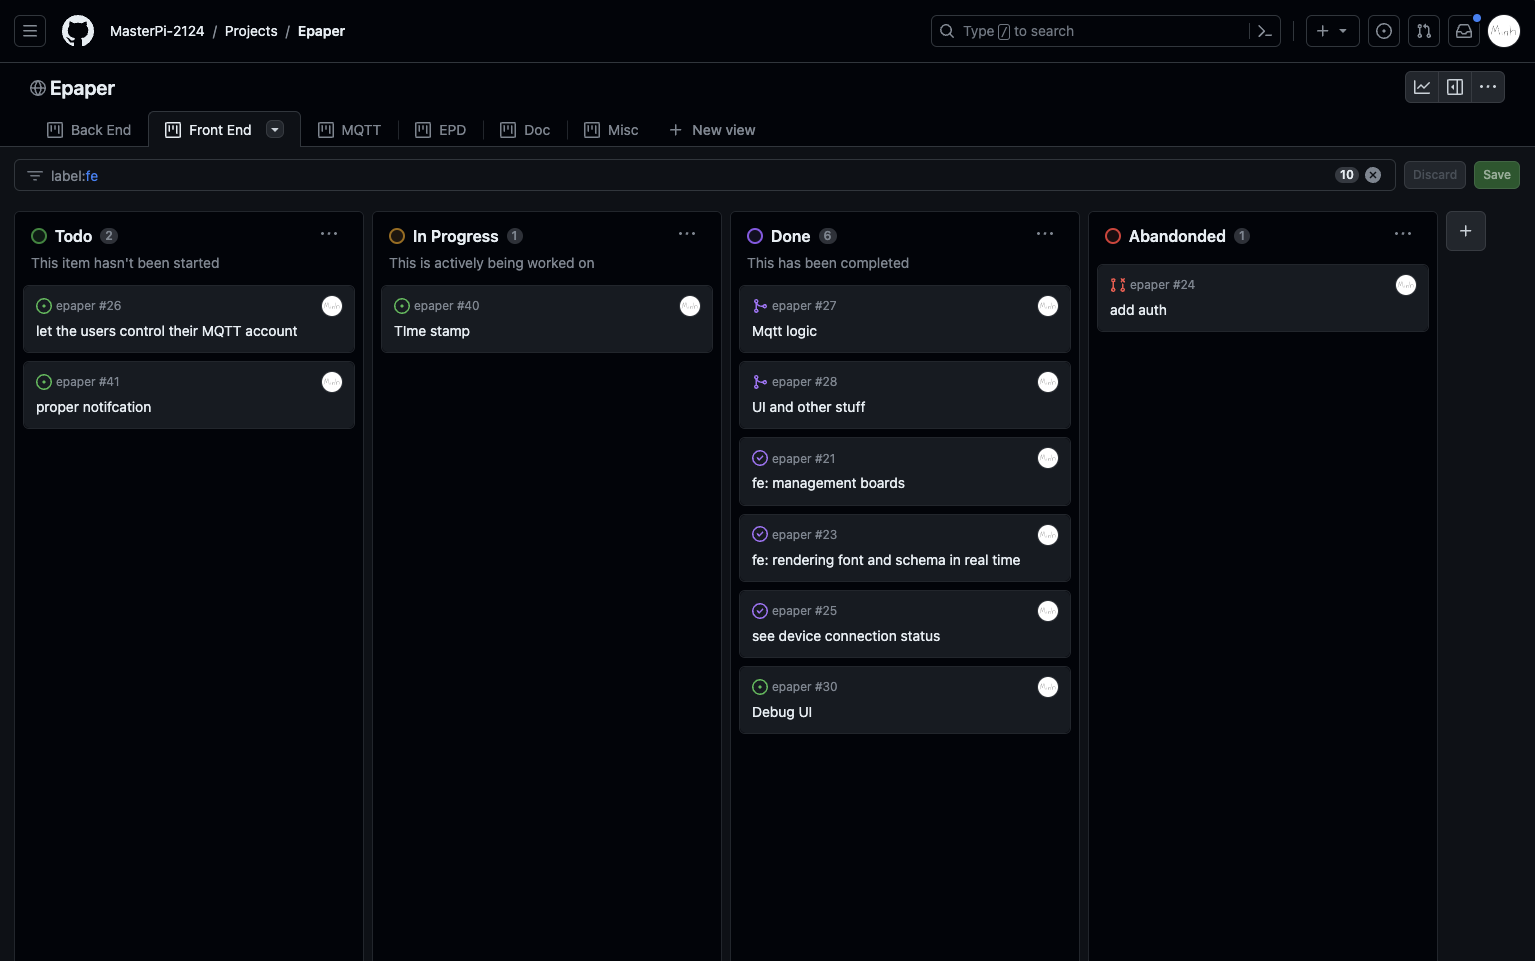
\includegraphics[width=0.8\linewidth]{doc//imgs/github-projects.png}
    \caption{Repository's Project screen}
    \label{fig:enter-label}
\end{figure}

\subsection{Achievement}
With the help of tools and libraries in the table \ref{fig:table_tools} above, the project has reached significant milestones and also released a minimum viable product (MVP), including the Management UI, the back-end server, and a couple of \gls{EPD} devices that can be implemented in many small business environments. While having some minor performance issues, this MVP still proved its usefulness in various use cases, such as mini-markets, schools, and offices, unveiling the enormous potential of the system in a broader spectrum of the service industry.

The whole system runs on the website, so the users don't need to install any additional applications. Also, the users only need to plug the \gls{EPD} device into the computer via a USB port when needed without additional drivers, and the website will automatically recognize the device. Details of the running system are shown in the table below.

\begin{table}[H]
    \newcolumntype{M}[1]{>{\centering\arraybackslash}m{#1}}
    \newcolumntype{L}[1]{>{\raggedright\arraybackslash}p{#1}}
    \renewcommand{\arraystretch}{3} % Adjust for row height
    \centering{}
    \fontsize{9pt}{8pt}\selectfont 
    \begin{tabular}{| m{3.5cm} | m{9cm} |}
        \hline
        \textbf{Description}    & \textbf{URL}                                          \\ \hline
        Management UI           & \url{https://epaper.artsakh.ventures}                 \\ \hline
        MongoDB Databases       & \url{mongodb://mongo.epaper.artsakh.ventures:27017}   \\ \hline
        Back-end server         & \url{https://epaper.artsakh.ventures/api}             \\ \hline
        MQTT Broker             & \url{mqtts://mqtt.epaper.artsakh.ventures:8883}       \\ \hline
        MQTT Management UI      & \url{https://epaper.artsakh.ventures/rabbitmq}        \\ \hline
        OpenAPI Swagger         & \url{https://epaper.artsakh.ventures/api/swagger}        \\ \hline
    \end{tabular}
    \caption{Project service URLs}
    \label{fig:table_tools}
\end{table}

The \gls{EPD} device consists of an ESP32-C3 Supermini development board with a Waveshare 2.9-inch e-paper display panel and is packaged inside a custom 3D printed case \footnote{Special thanks to MSc. Nguyen Duc Tien for the 3D-printed case and the packaged EPD device}. The battery powering the system is a 135mAh Lithium-ion battery and is rechargeable via the USB-C port of ESP32-C3.

\subsection{Illustration of main functions}
To manage \gls{EPD} Devices and data, users have to log in with credentials as illustrated in the image \ref{fig:login-screen}. After logging in, the user can choose to create data/device or go to the dashboard to manage them by choosing the pages from the left sidebar, which is shown in figure \ref{fig:dashboard}. 
\begin{figure}[H]
    \centering
    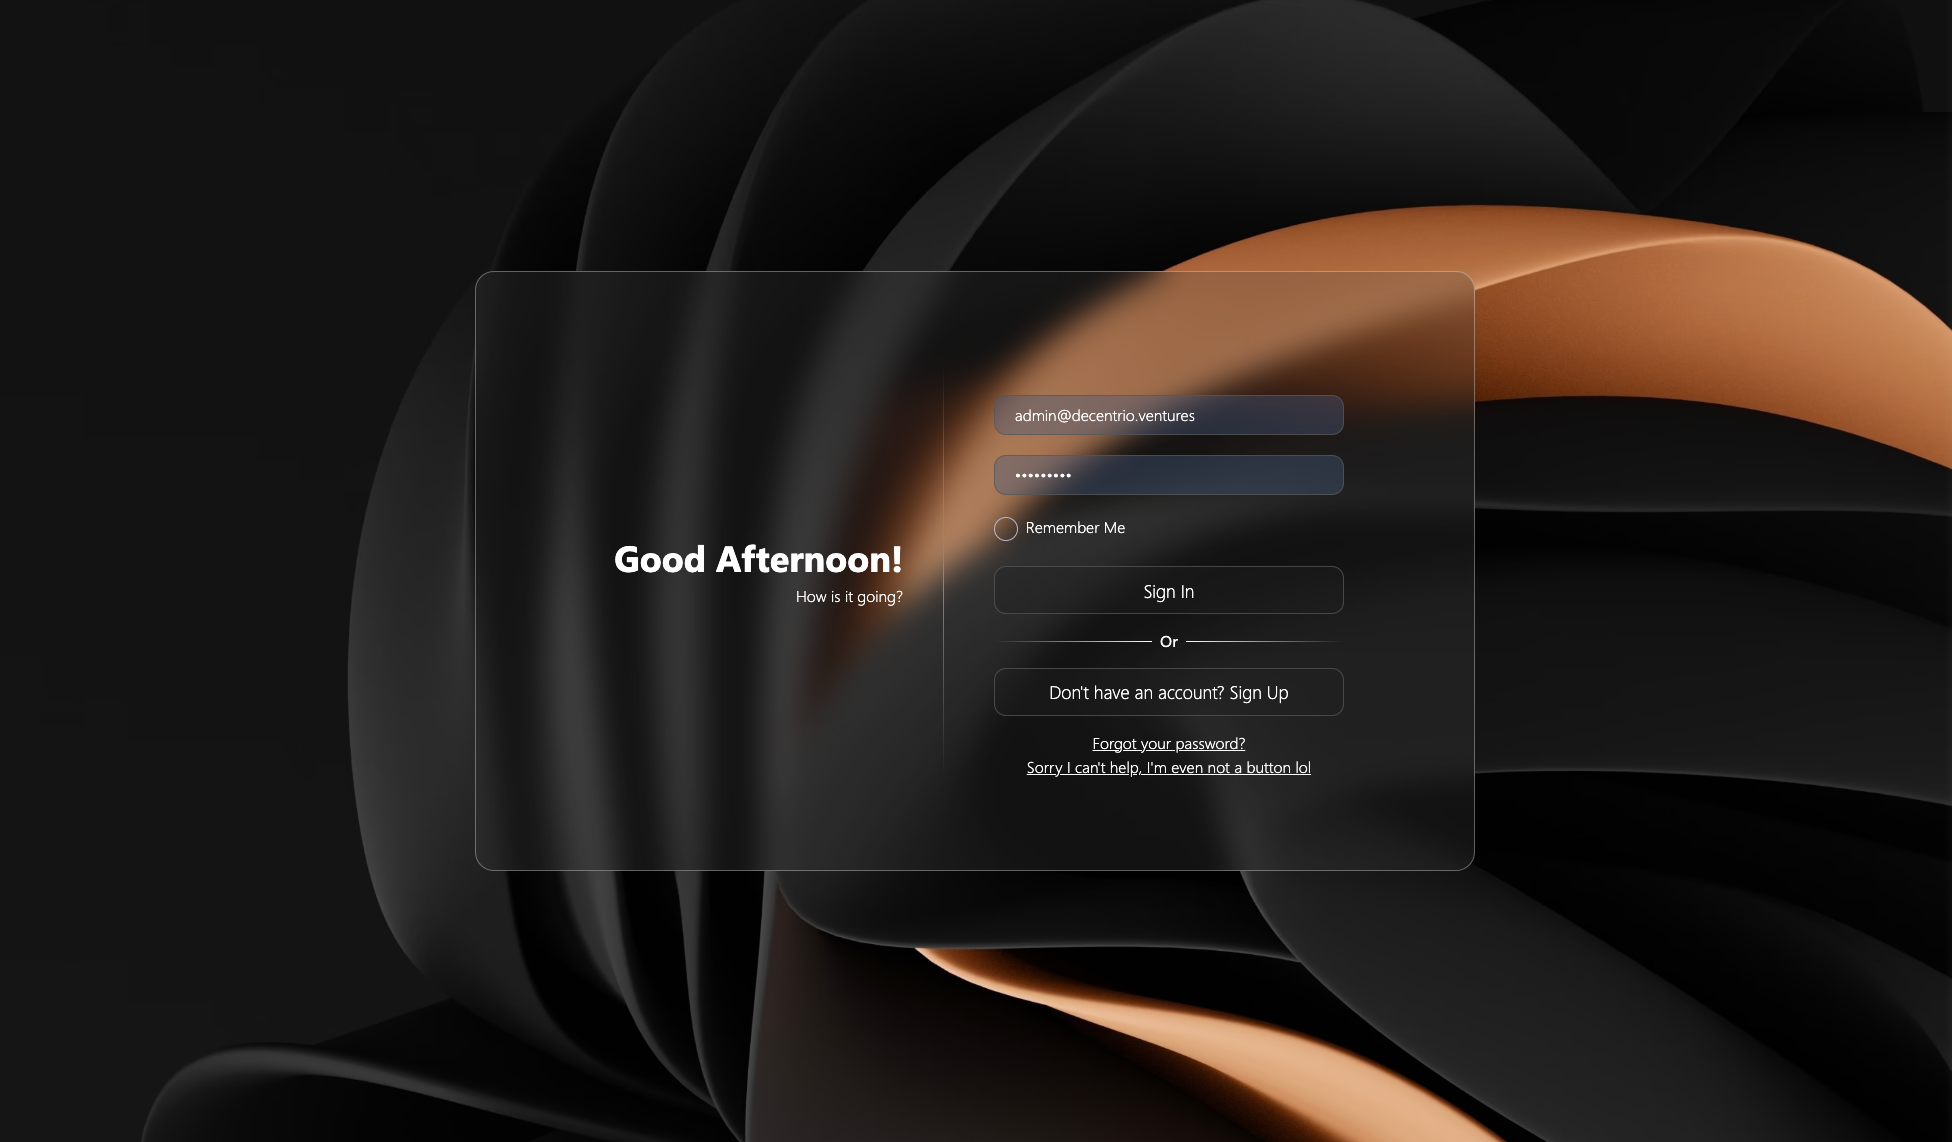
\includegraphics[width=0.8\linewidth]{doc//imgs/ui_login.png}
    \caption{Login screen}
    \label{fig:login-screen}
\end{figure}

\begin{figure}[H]
    \centering
    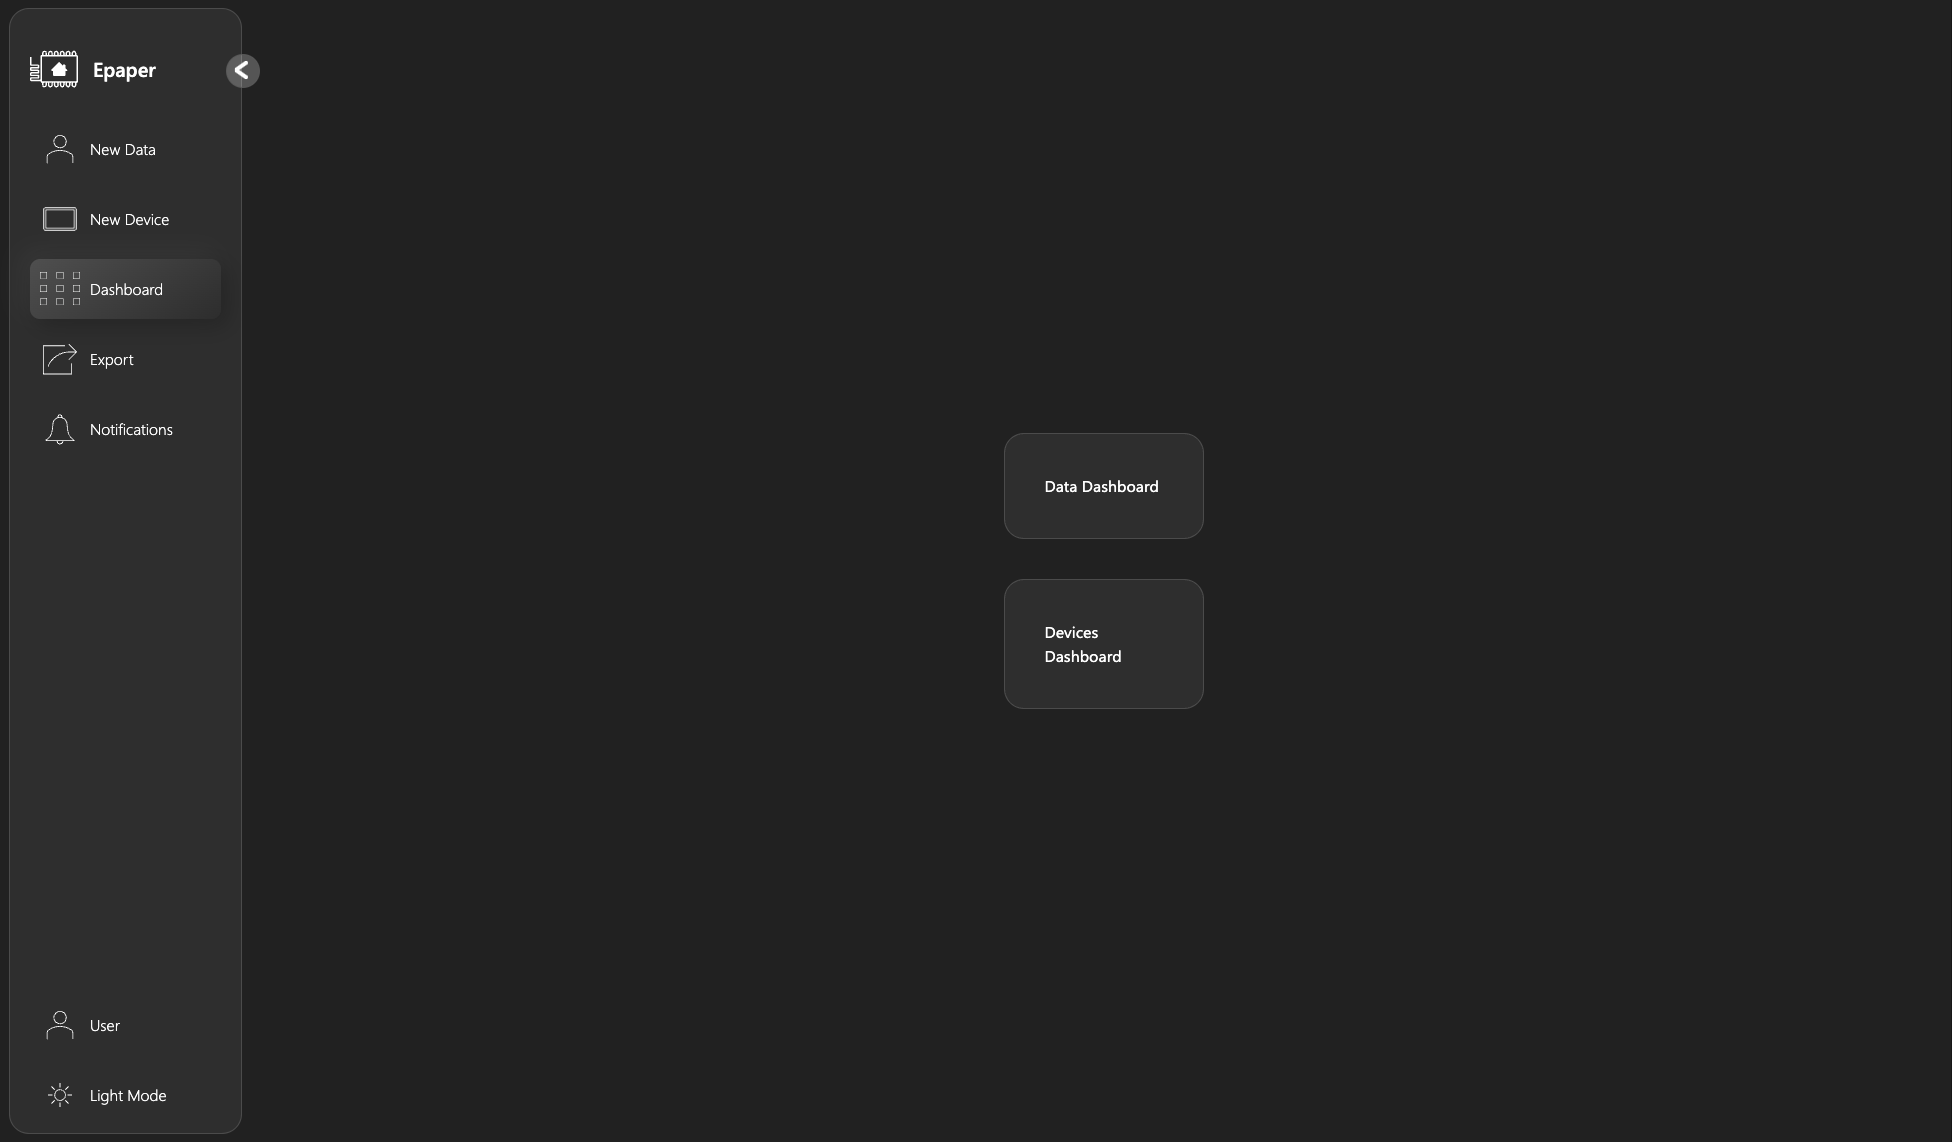
\includegraphics[width=0.8\linewidth]{doc//imgs/ui_dashboard.png}

    \caption{Dashboard Screen}
    \label{fig:dashboard}
\end{figure}

\begin{figure}[H]
    \centering
    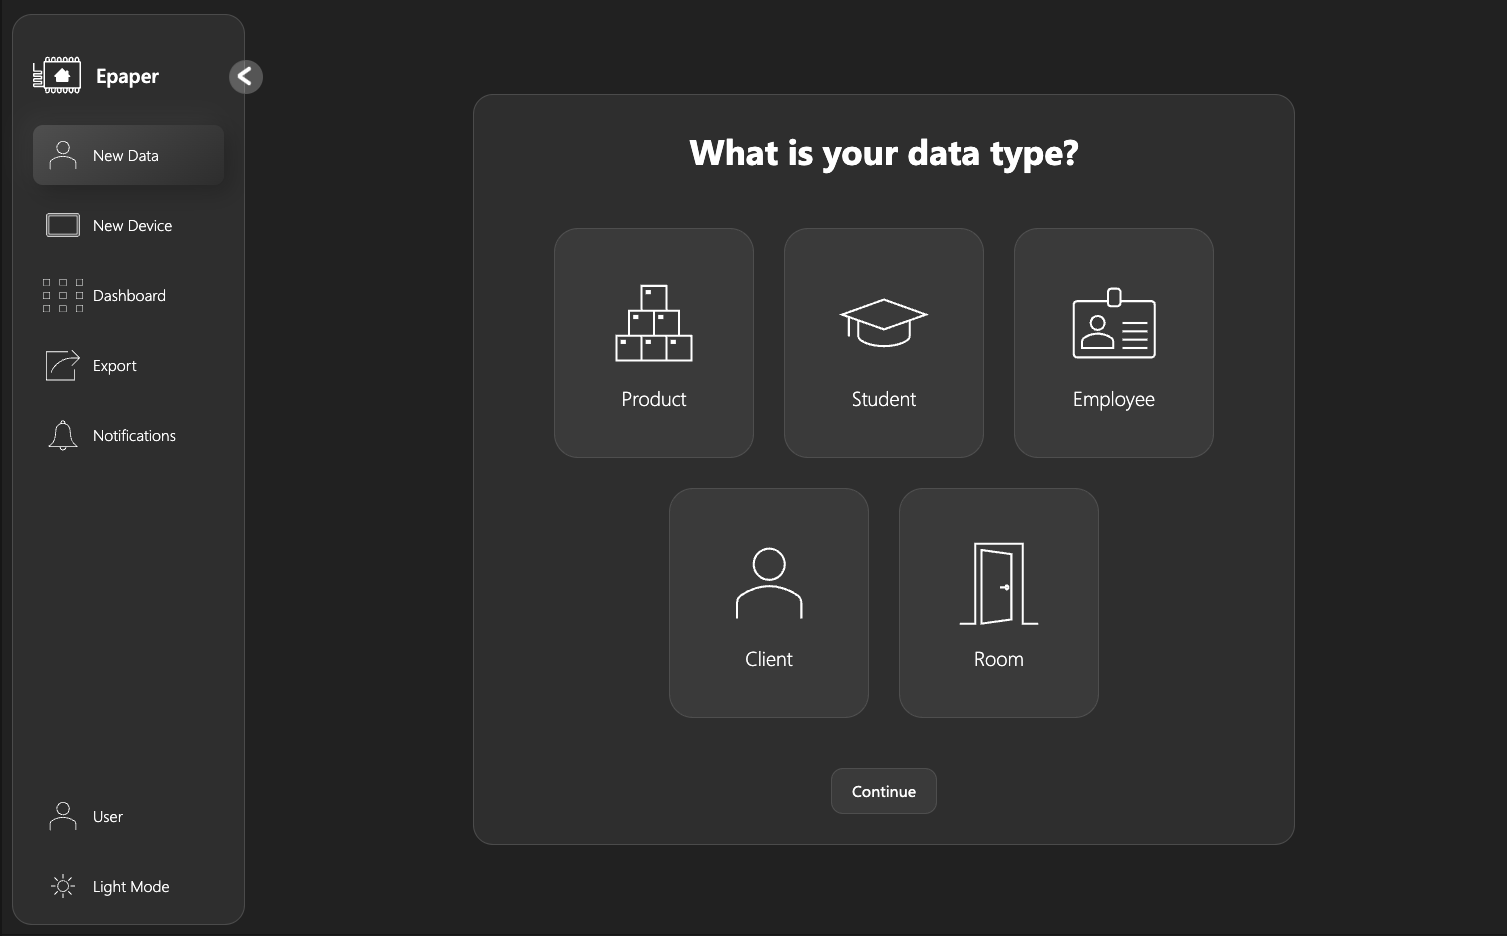
\includegraphics[width=0.95\linewidth]{doc//imgs/ui_new-data-type.png}
    \caption{"Choose data type" screen in "New Data"}
    \label{fig:new-data-type}
\end{figure}


When creating data, the user can easily follow on-screen instructions and fill in the required information. All the steps are annotated in detail, and the rendered display is showing in real-time, which helps improve user experience. Figure \ref{fig:new-data-type} below illustrates the process of creating new data at the data type step, which requires users to choose the type of data before providing more detail and going to the device-choosing step shown in figure \ref{fig:new-data}. The user can select the active device and their preferred display configurations and see the pre-rendered display of the data.
\begin{figure}[H]
    \centering
    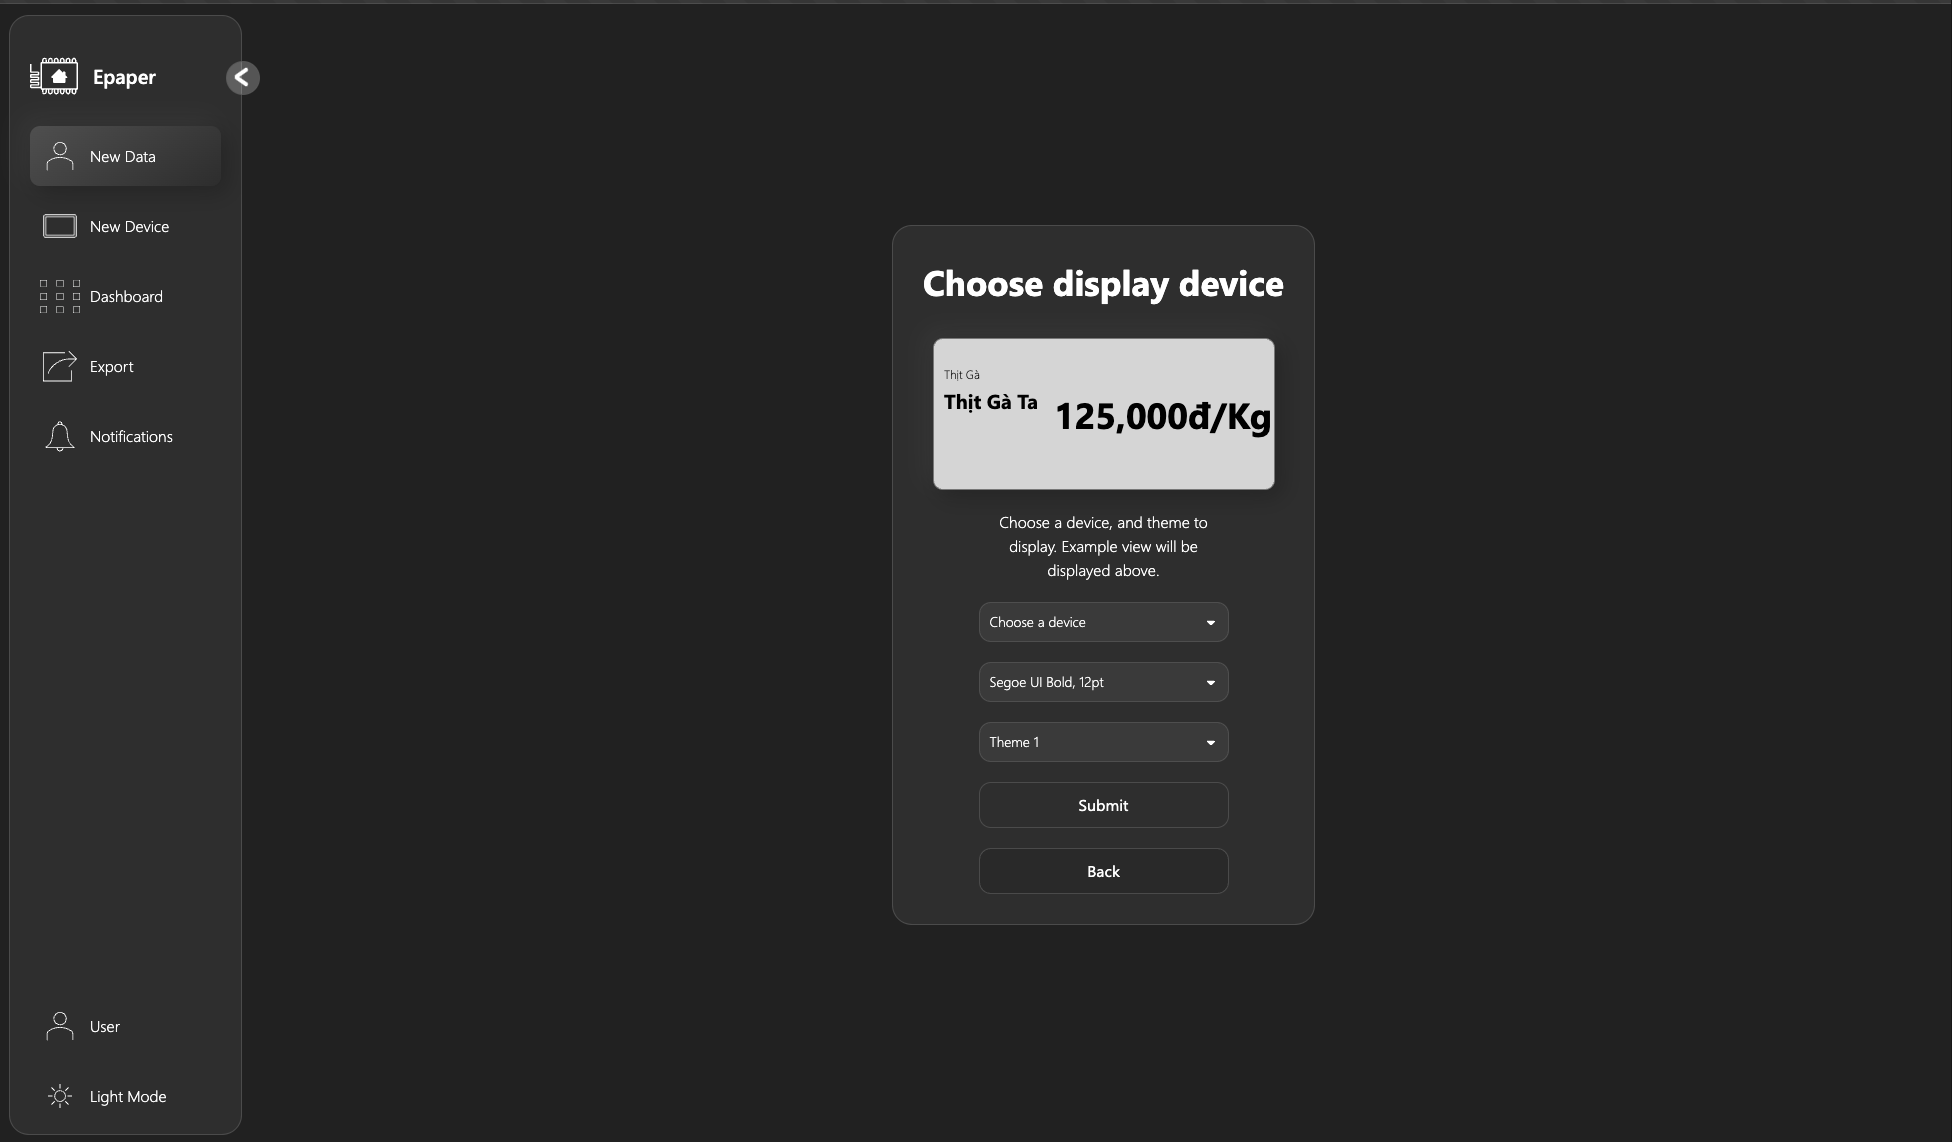
\includegraphics[width=0.95\linewidth]{doc//imgs/ui_new-data.png}
    \caption{"Choose device" screen in "New Data"}
    \label{fig:new-data}
\end{figure}

When registering a new device, users need to plug the \gls{EPD} device into the USB port of the PC they are using. Then, users can choose the device from the connected devices list and provide its name and Wi-Fi credentials before submitting it to the system.

\begin{figure}[H]
    \centering
    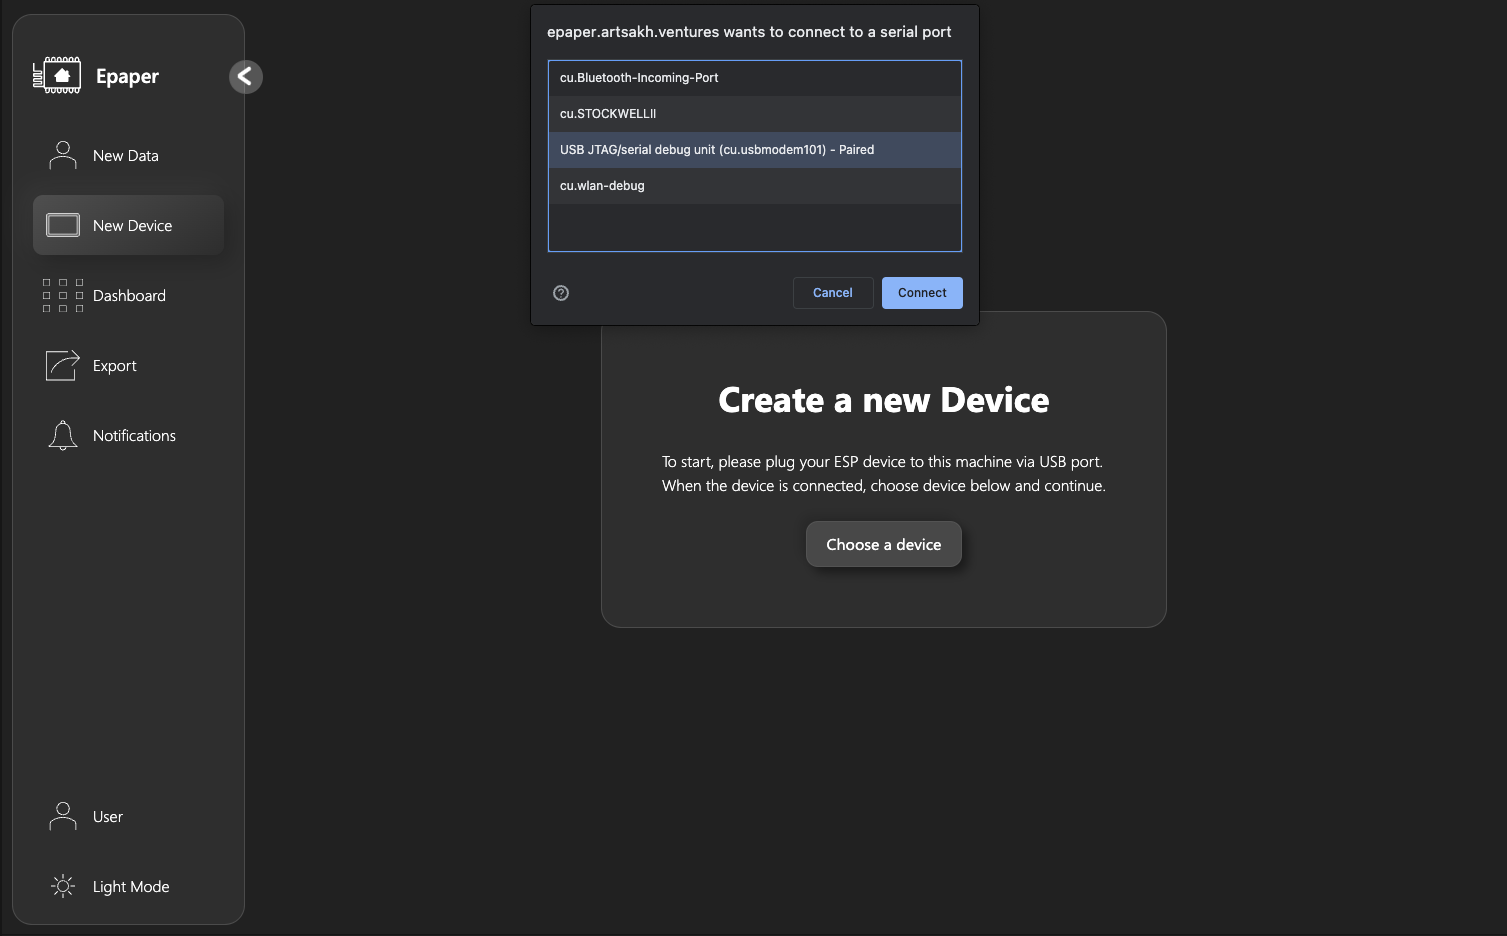
\includegraphics[width=0.87\linewidth]{doc//imgs/ui_new-device.png}
    \caption{"New Device" page}
    \label{fig:ui_new-device}
\end{figure}

In the device's dashboard, the users can see information together with the status of each device and also can choose to view more detail, edit, or delete devices via the buttons on the right side. Figure \ref{fig:detail-modal} below shows the detailed modal of an active device displaying the data. 

\begin{figure}[H]
    \centering
    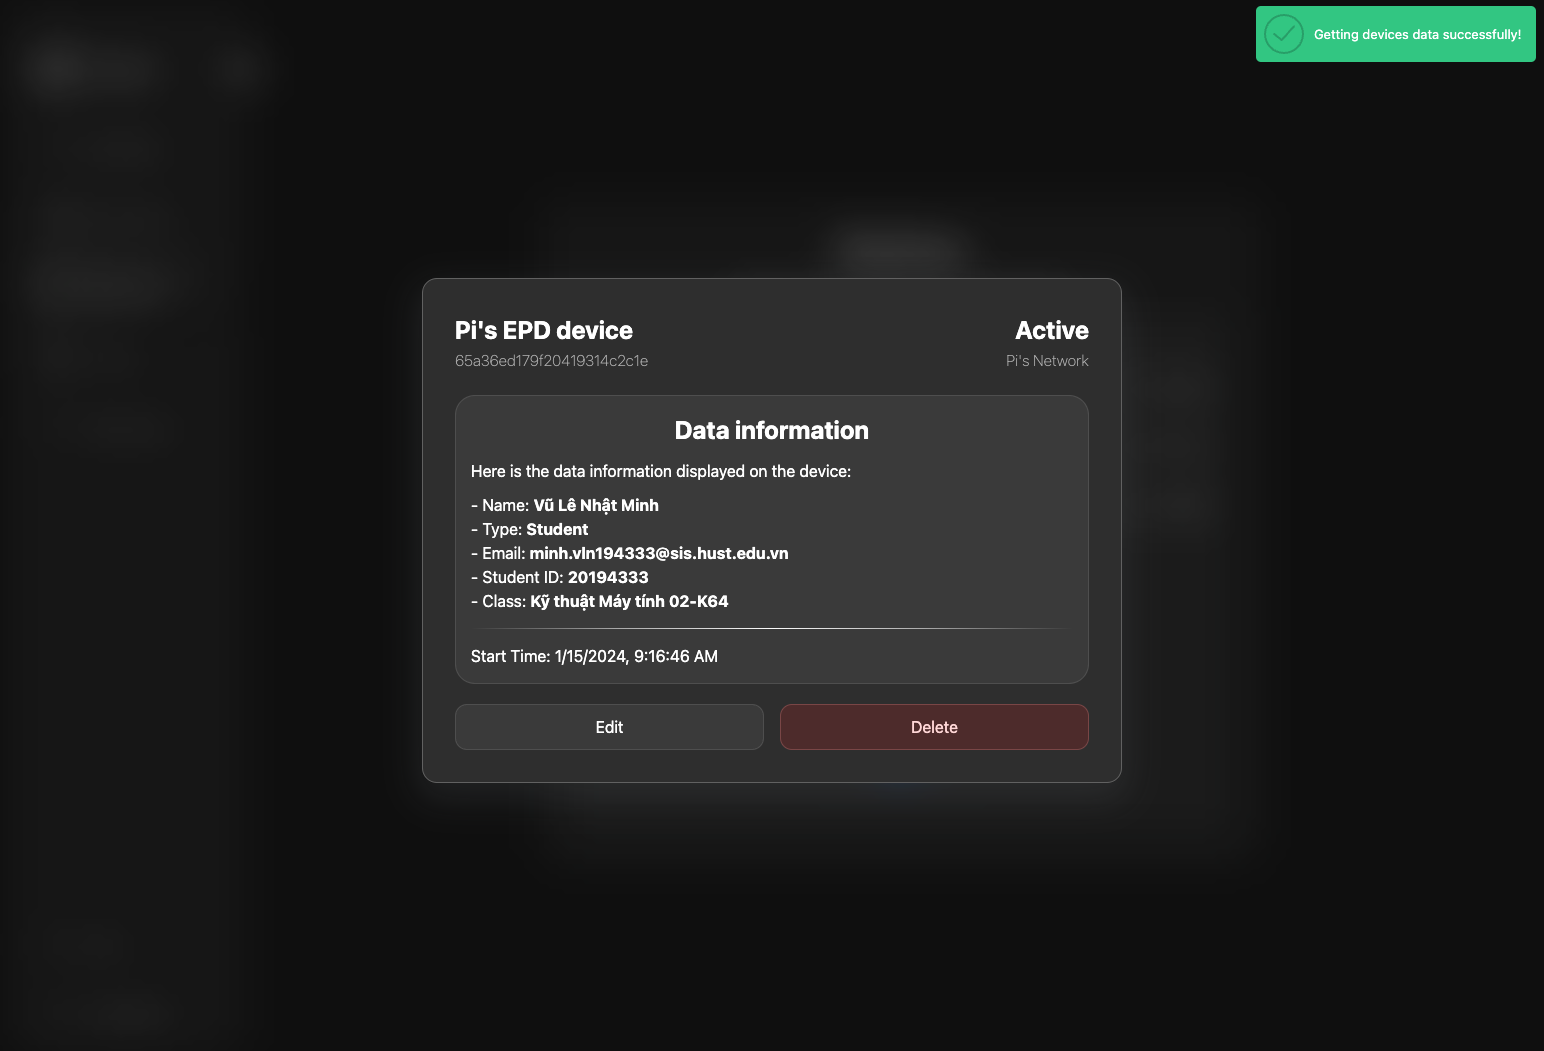
\includegraphics[width=0.85\linewidth]{doc//imgs/ui_device-modal.png}
    \caption{Detail modal of an active device displaying data}
    \label{fig:detail-modal}
\end{figure}

The users can also check the serial output of the device via Serial Port and even pop it out into the PiP component by choosing the "Show log (debug)" button (figure \ref{fig:ui_debug}), which enables them to test interacting with the device right on the website while still monitoring the device's log (figure \ref{fig:data-dashboard}). This feature is handy in case some problems occur on the device and users don't have the proper instruments to debug further. Moreover, users can also upgrade the devices wirelessly by choosing the "OTA Uprgade" feature and choosing the \verb|.bin| binary file, which is illustrated in figure \ref{fig:ui_firmware} below. The server will receive the binary file and send an OTA request to the assigned device.

\begin{figure}[H]
    \centering
    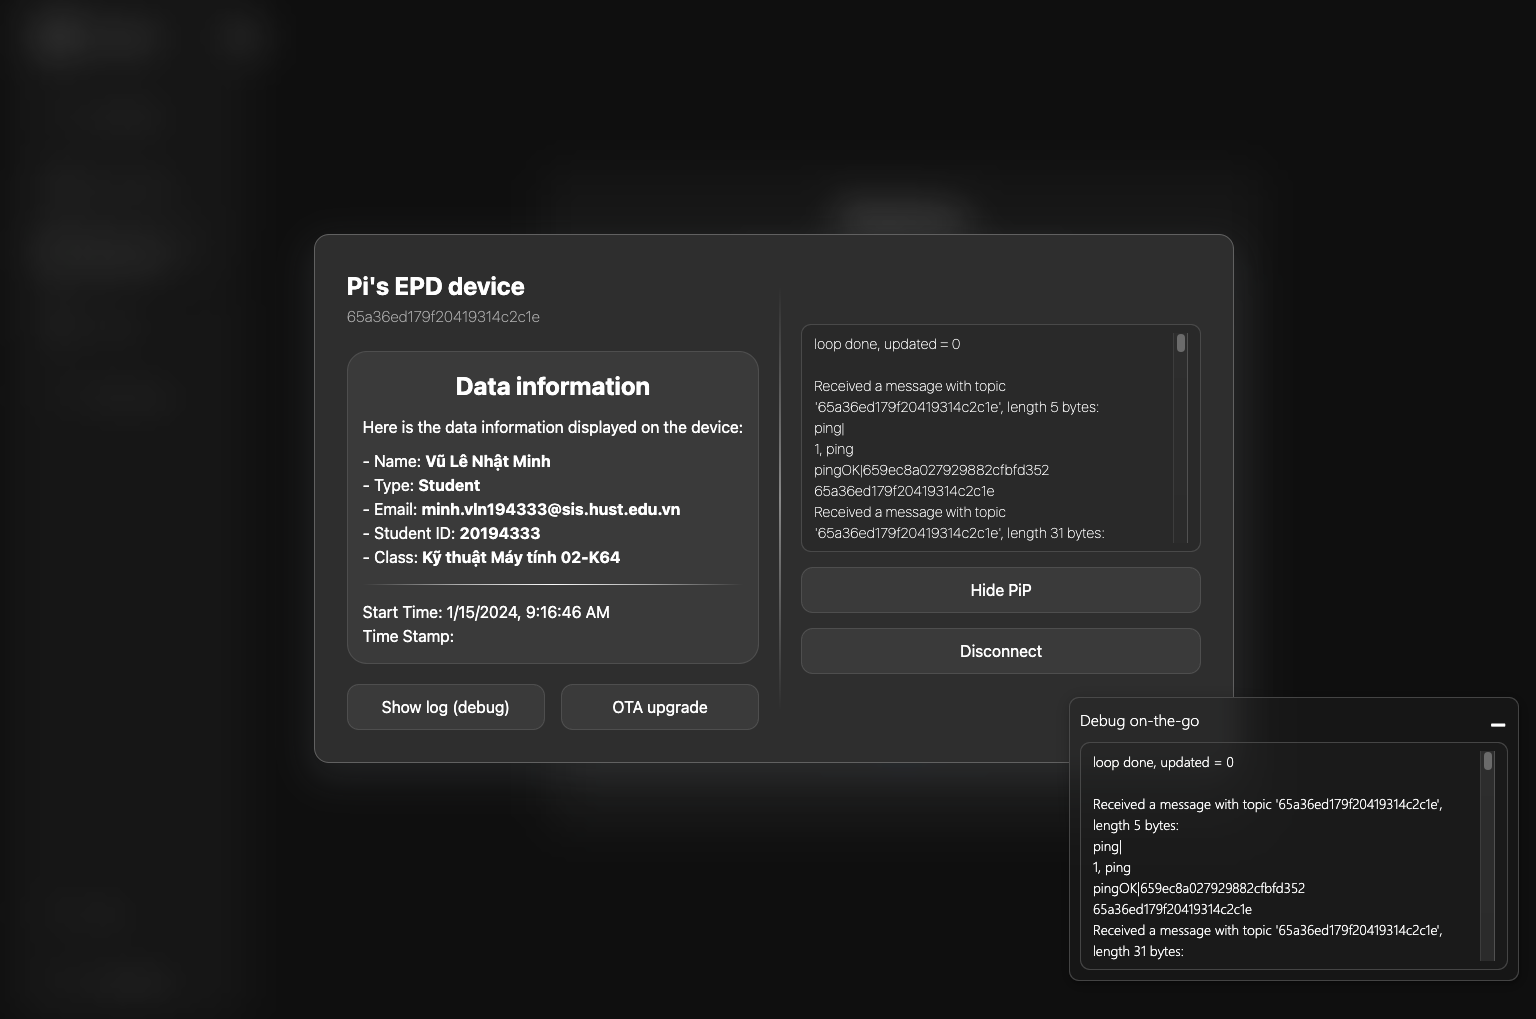
\includegraphics[width=0.85\linewidth]{doc//imgs/ui_debug.png}
    \caption{Debug modal showing the log of the device}
    \label{fig:ui_debug}
\end{figure}

\begin{figure}[H]
        \centering
        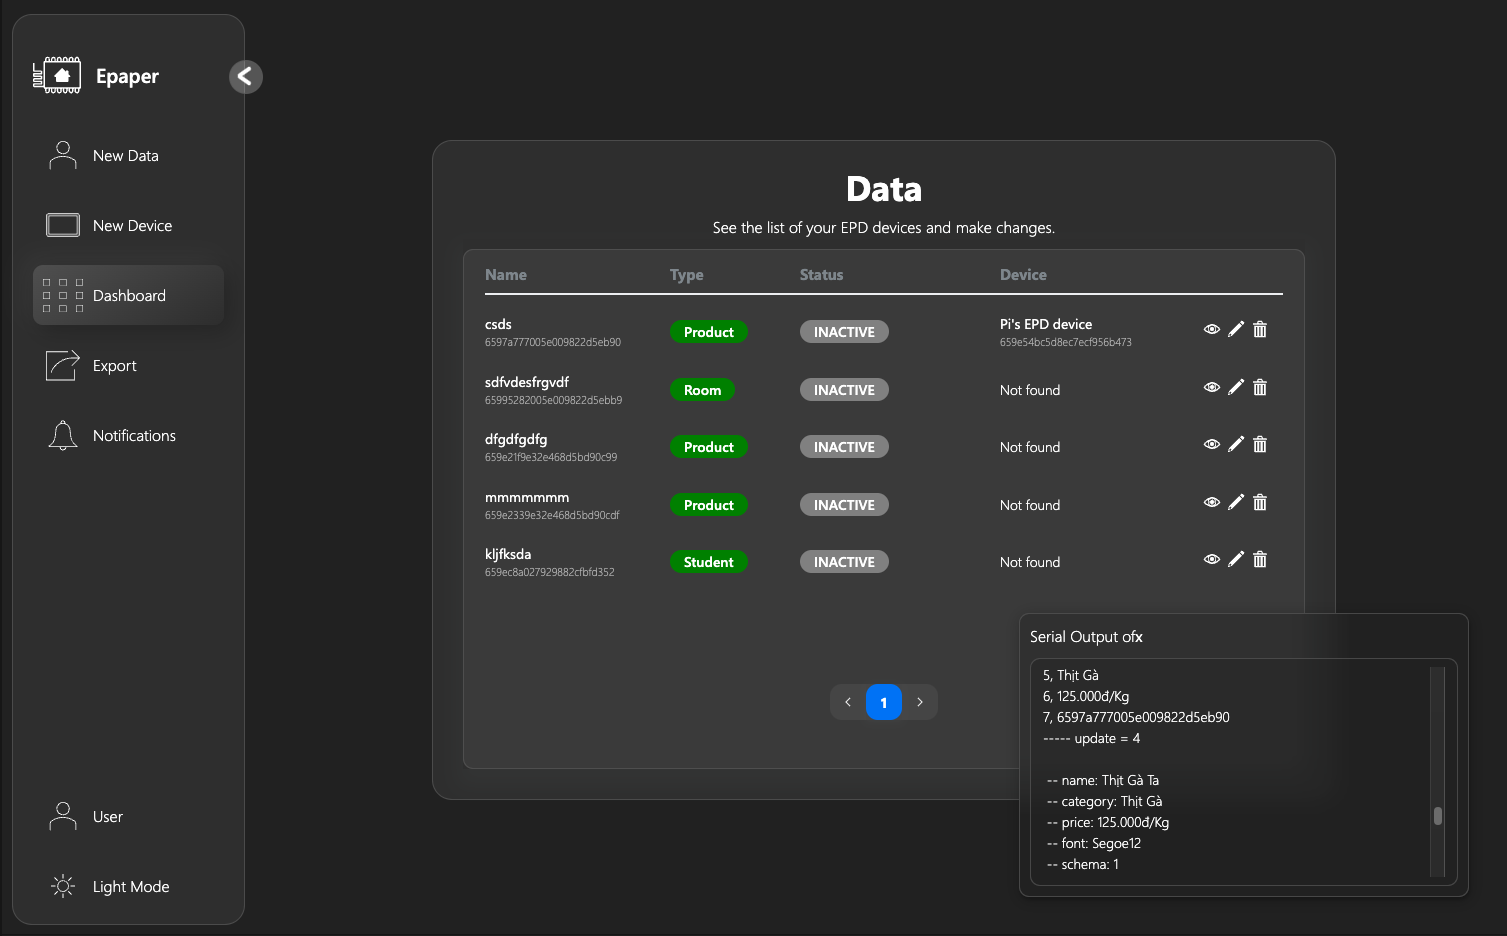
\includegraphics[width=0.85\linewidth]{doc//imgs/ui_data-dashboard.png}
        \caption{Data dashboard, with a PiP showing device log}
        \label{fig:data-dashboard}
\end{figure}

\begin{figure}[H]
    \centering
    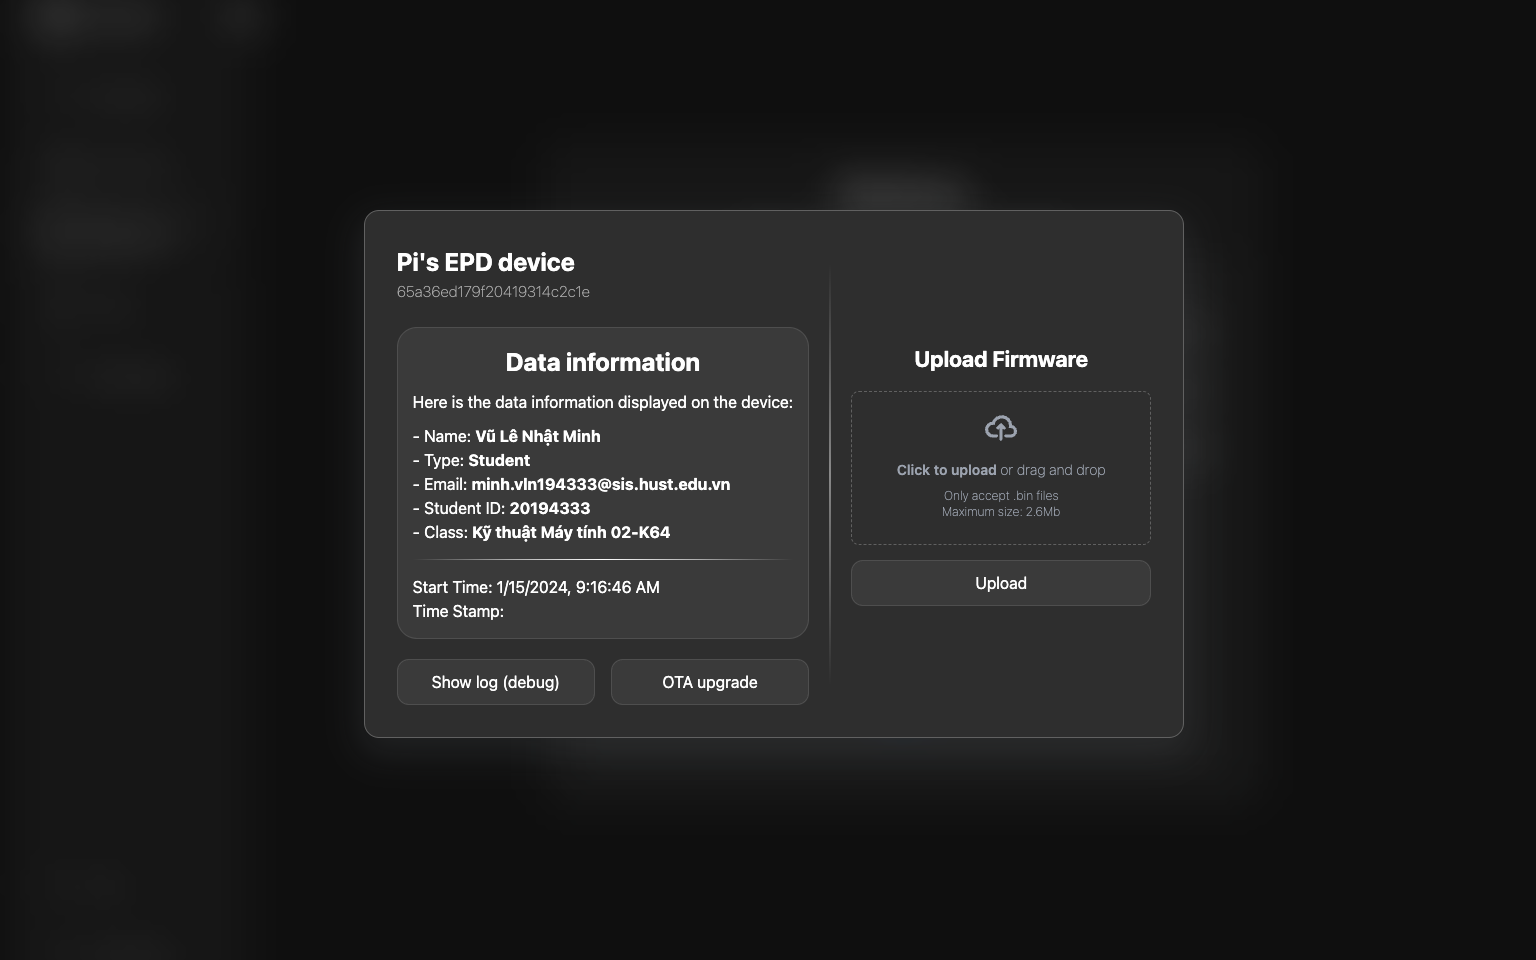
\includegraphics[width=0.82\linewidth]{doc//imgs/ui_firmware.png}
    \caption{Debug modal showing firmware upload section}
    \label{fig:ui_firmware}
\end{figure}

The \gls{EPD} Device connects to the MQTT Broker and subscribes to its ID as the topic. The picture \ref{fig:epd_no-data} on the left side below indicates the device display when no data is stored, and \ref{fig:epd_name} on the right side shows the device display when data is stored and displayed in the device. 

\begin{figure}[H]
  \centering
  \begin{minipage}[b]{0.45\textwidth}
    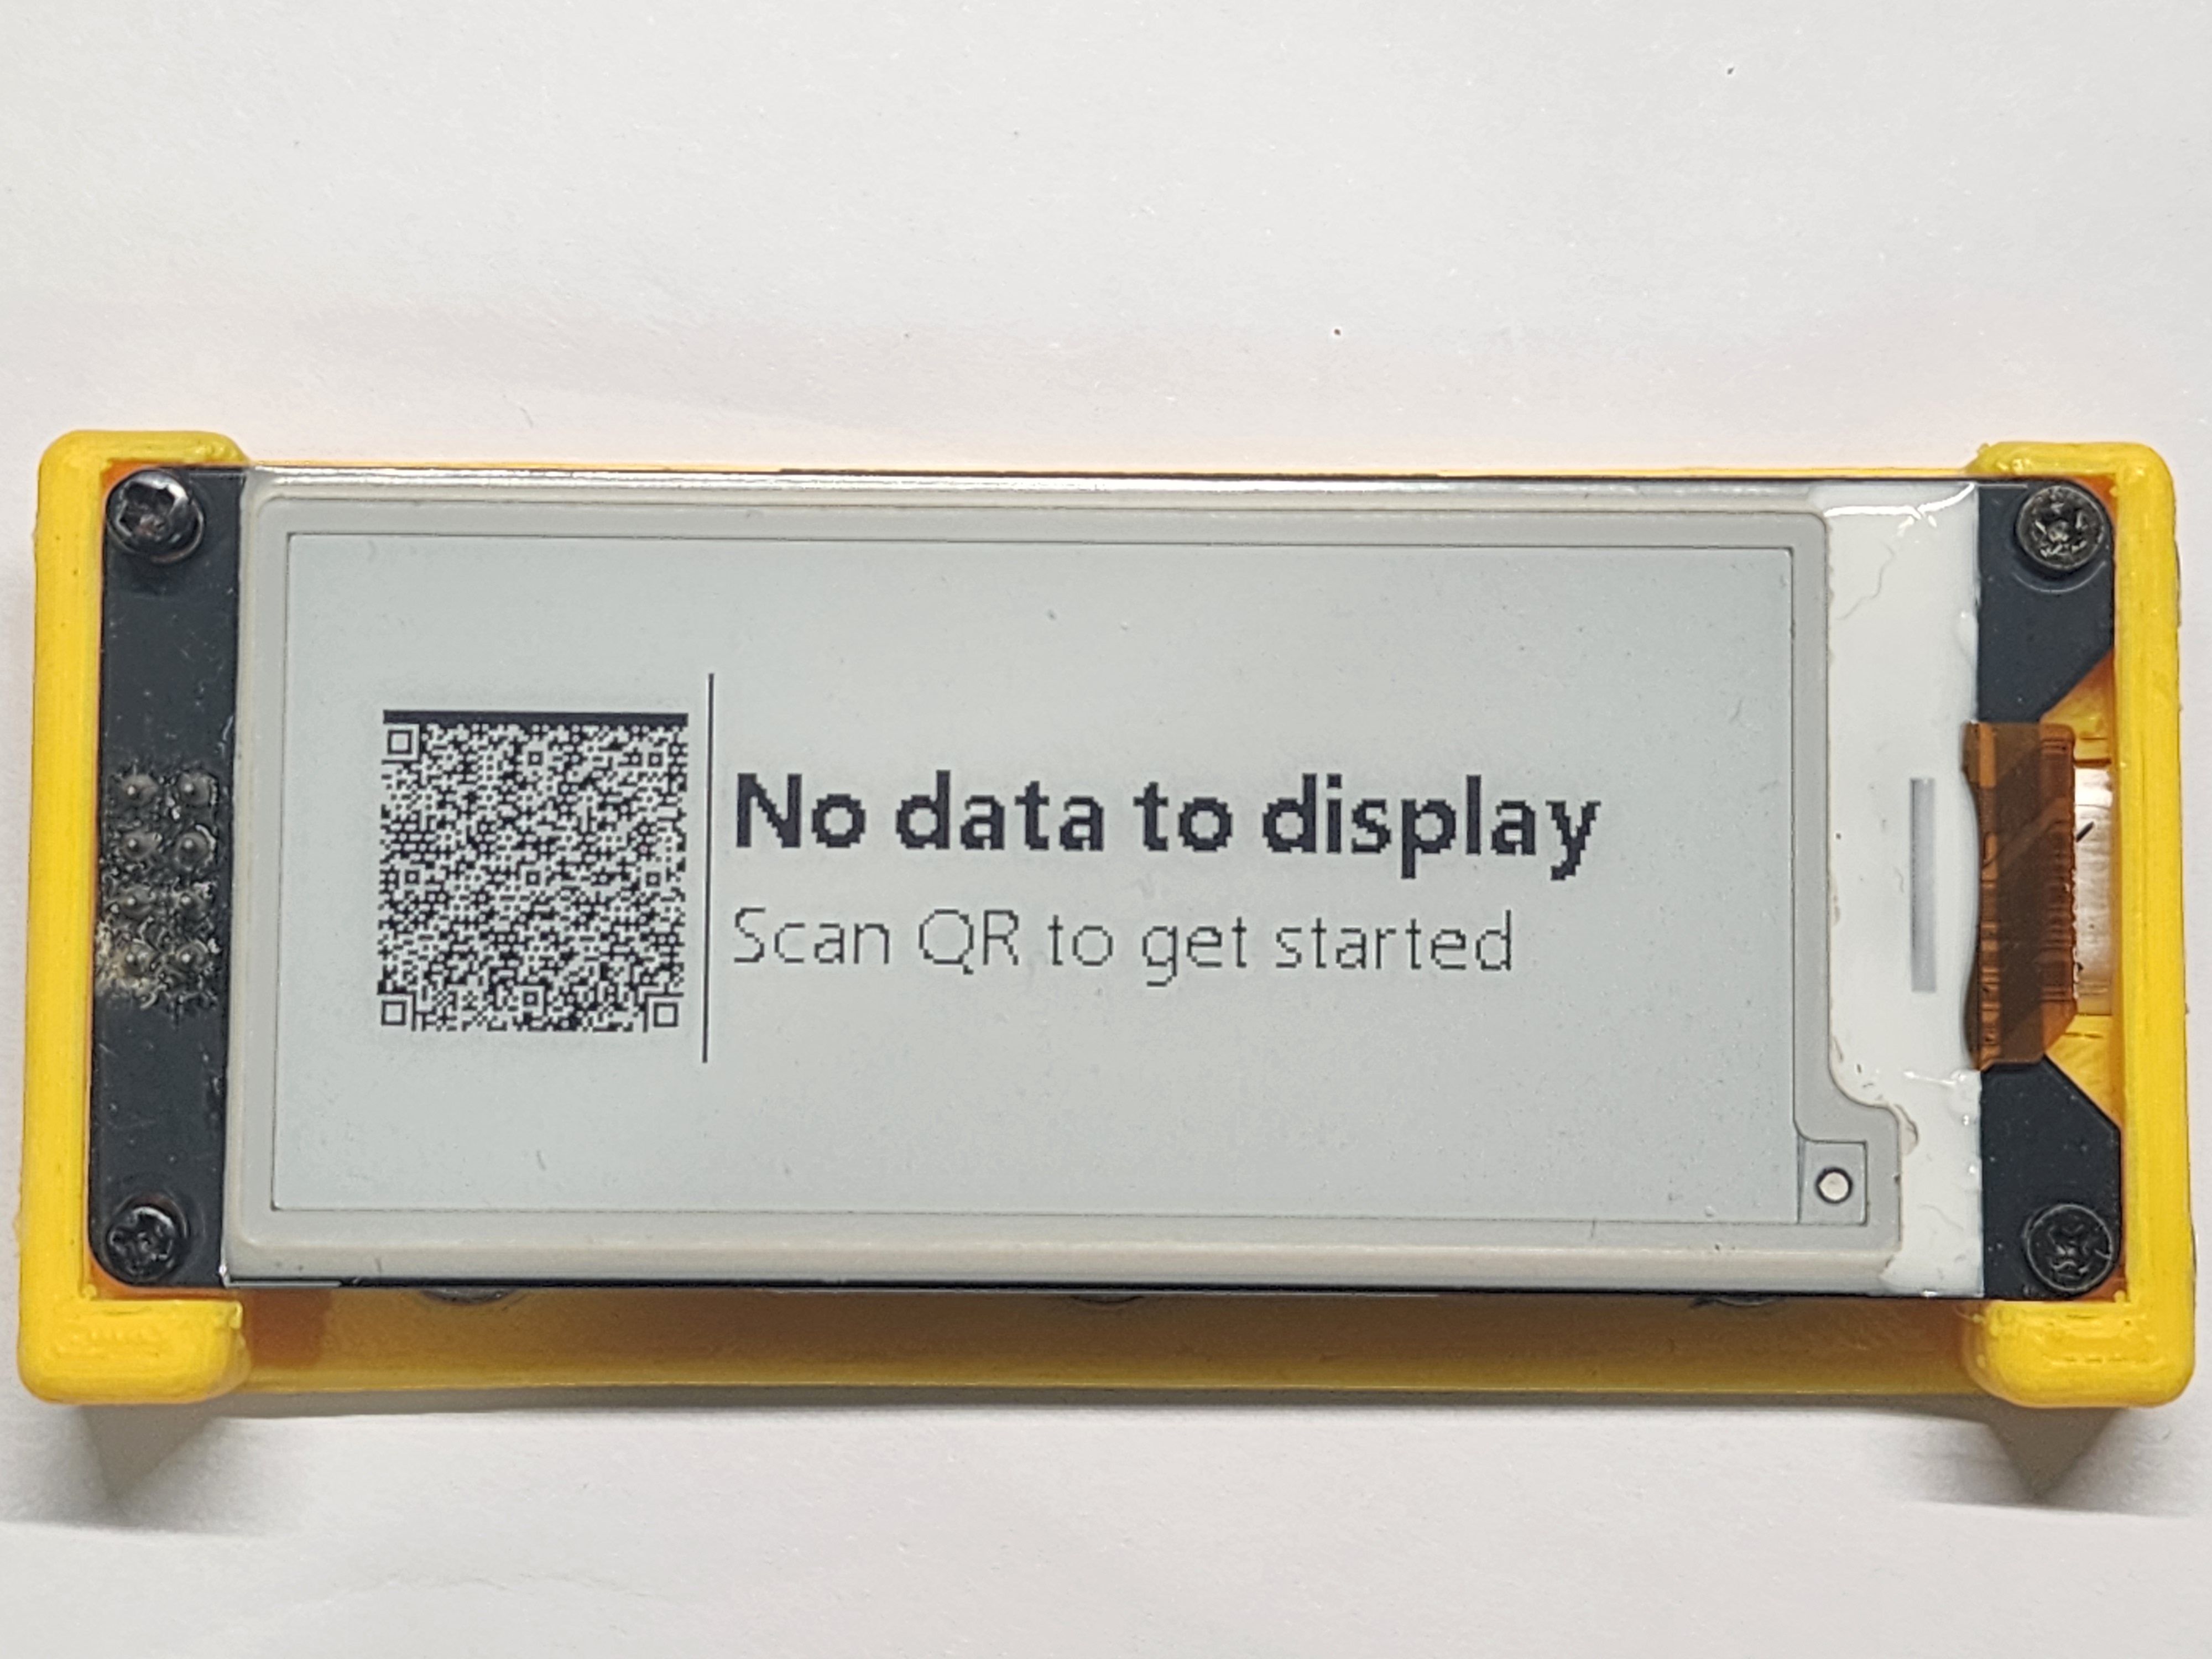
\includegraphics[width=\textwidth]{doc//imgs/epd_no-data.png}
    \caption{EPD display when no data is received}
    \label{fig:epd_no-data}
  \end{minipage}
  \hfill
  \begin{minipage}[b]{0.45\textwidth}
    \includegraphics[width=\textwidth]{doc//imgs/epd_name.png}
    \caption{EPD display when displaying a student data}
    \label{fig:epd_name}
  \end{minipage}
\end{figure}

Users can also put the \gls{EPD} device in debugging mode to test the devices. Currently, to do so, users need to hold the "Boot" button on the ESP32-C3 for 5 seconds, and it will reboot to the debugging mode and test the functionalities of the screen (figure \ref{fig:epd_debug}). This access method is not user-friendly and is only temporary in the development of the project. The improvement to this, and also other improvements of the system in the future, are discussed in chapter \ref{chapter:Conclusion}.

\begin{figure}[H]
    \centering
    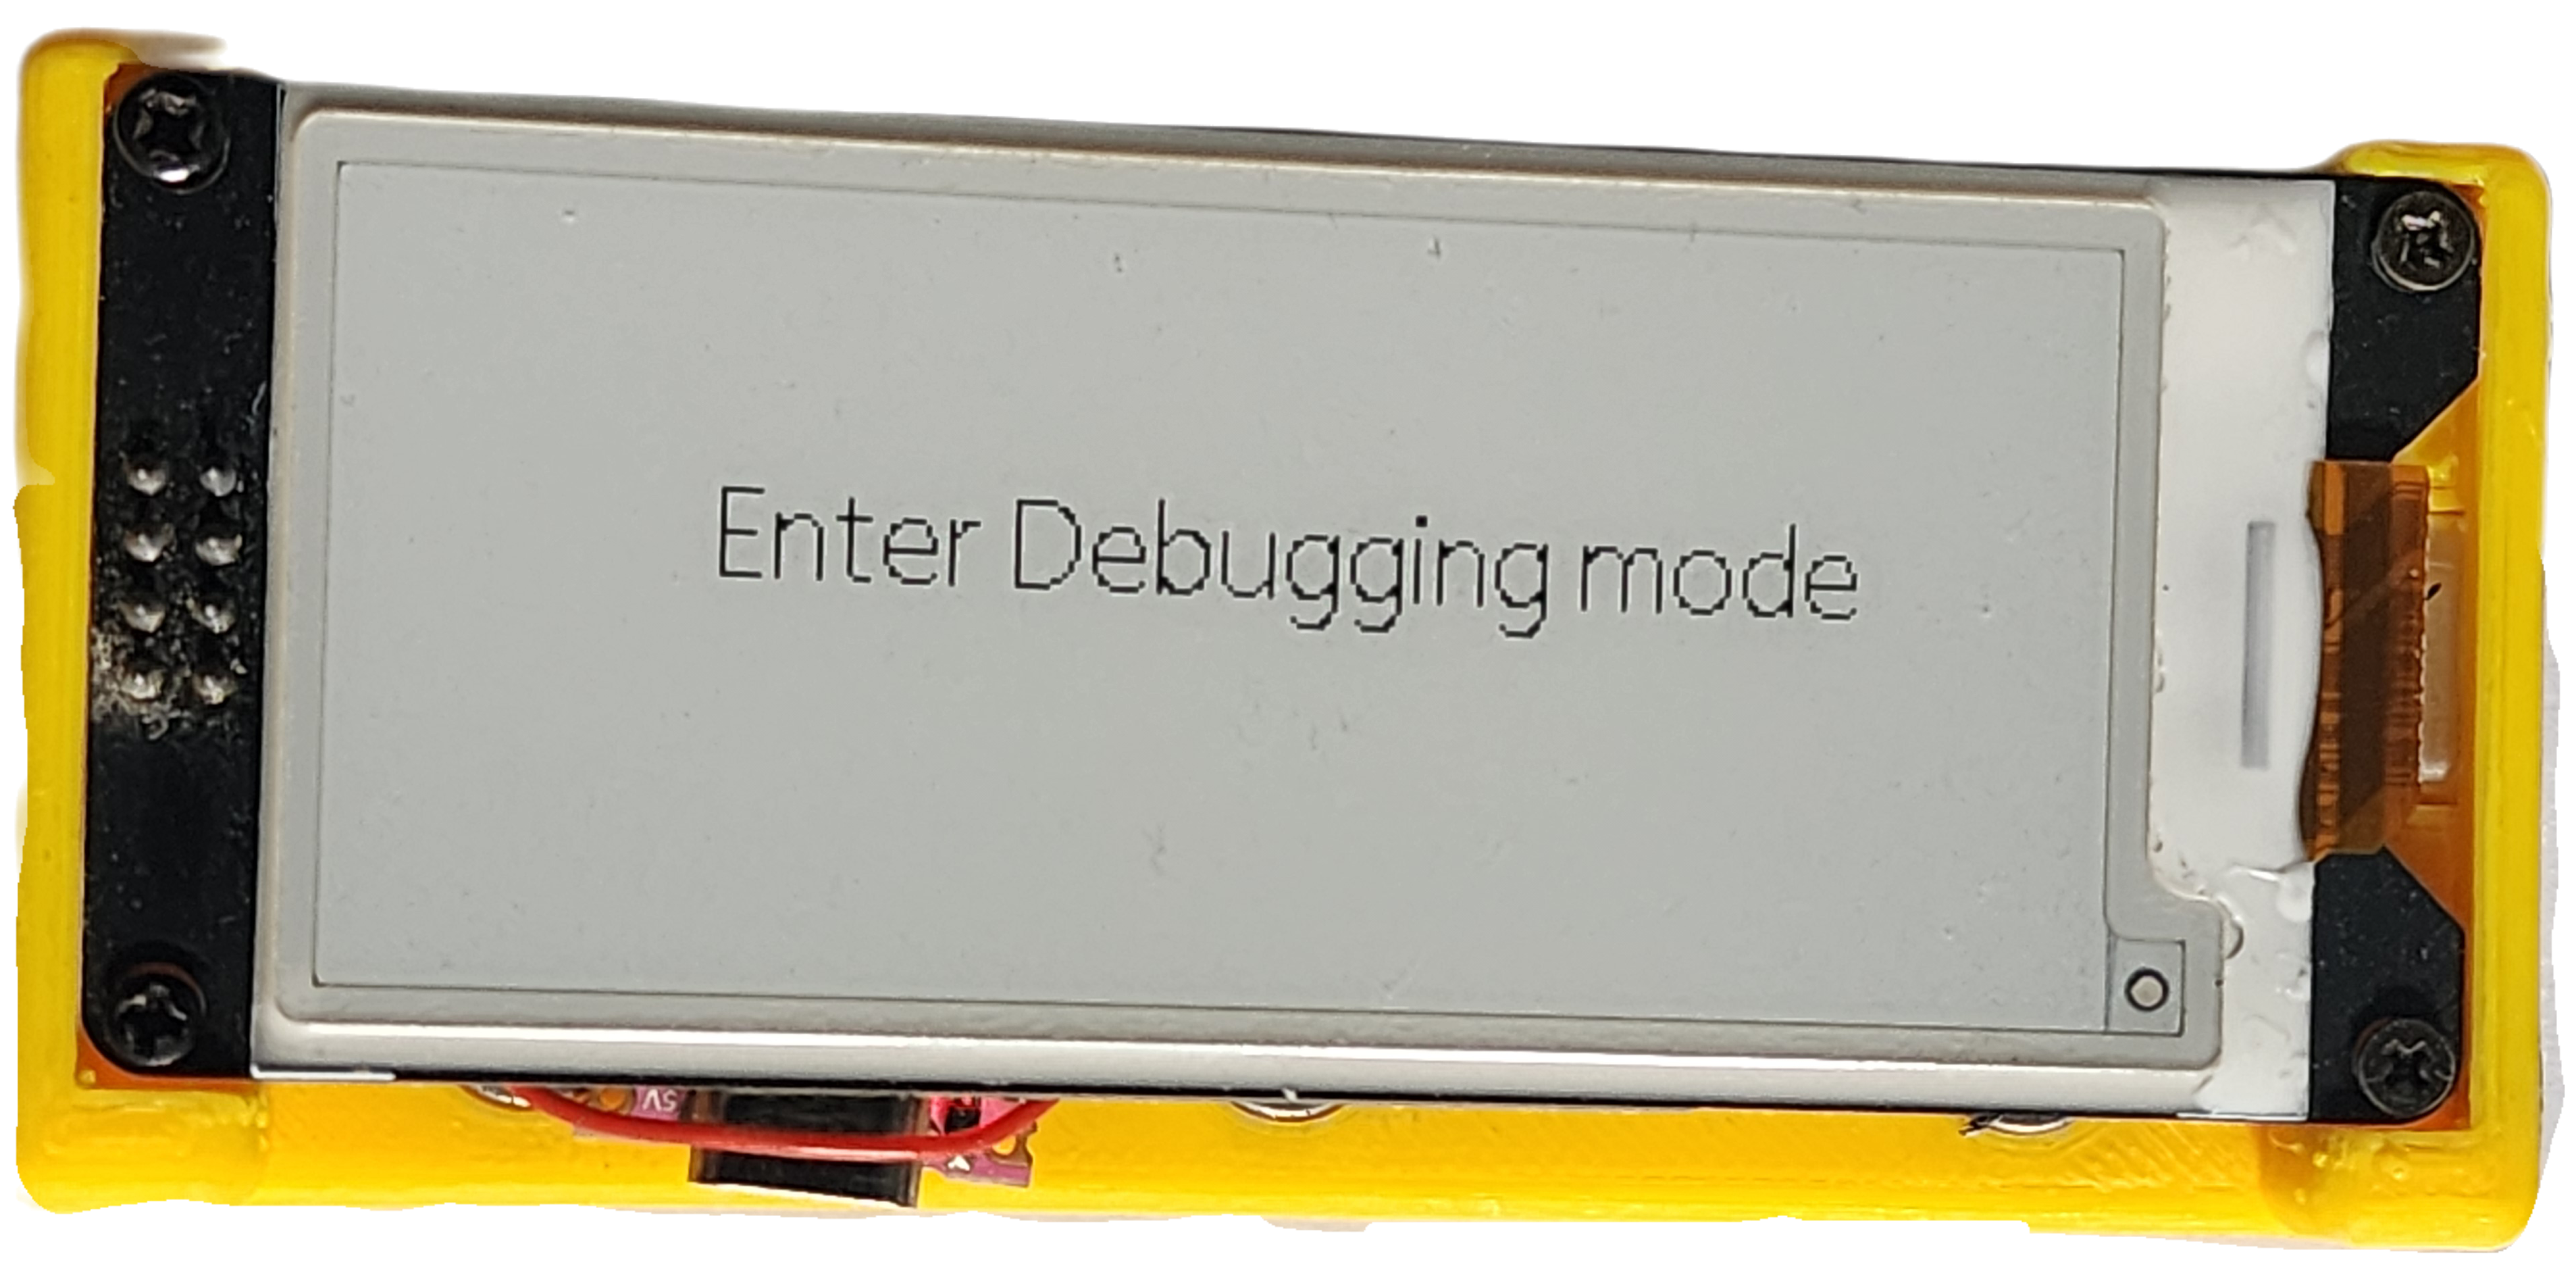
\includegraphics[width=0.7\linewidth]{doc//imgs/epd_debug.png}
    \caption{EPD device going to debug mode}
    \label{fig:epd_debug}
\end{figure}

\section{Testing and evaluation}
\subsection{Evaluation}
The project utilizes Lighthouse - an open-source tool by Google used for analyzing, measuring, improving quality, and optimizing the Management UI's performance. Lighthouse evaluates a web page's performance based on five criteria: performance, accessibility, best practices, search engine optimization (SEO), and Progressive Web App (PWA) compatibility\cite{lighthouse}. This tool not only provides a comprehensive analysis of web pages but also recommends ways to enhance the quality of the website. In this project, Progressive Web App (PWA) is not accounted for because the website only focuses mainly on desktop users. 

The results of the website quality assessment are shown in figure \ref{fig:ui_light-house}, and details are listed in table \ref{fig:ligthhouse-report}.
\begin{figure}[H]
    \centering
    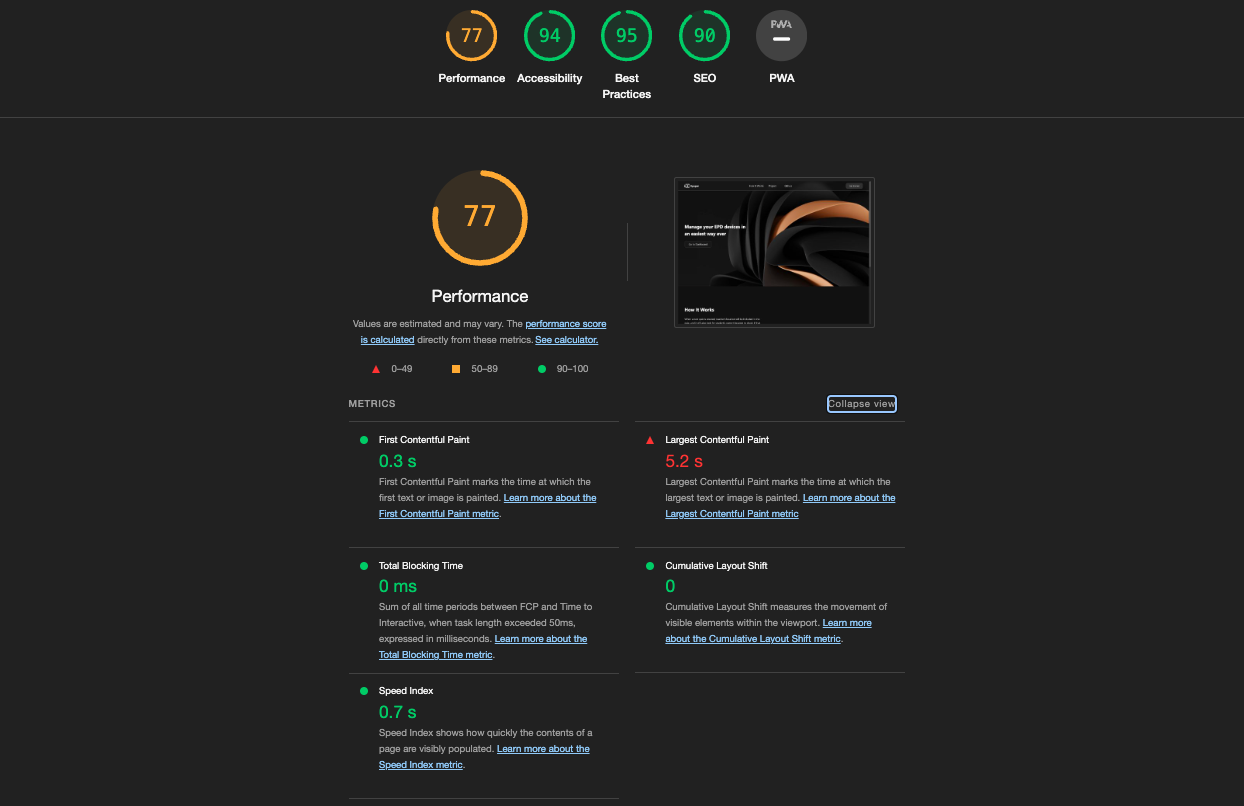
\includegraphics[width=0.8\linewidth]{doc//imgs/ui_light-house.png}
    \caption{Performance reports by Lighthouse}
    \label{fig:ui_light-house}
\end{figure}

\begin{table}[H]
    \newcolumntype{M}[1]{>{\centering\arraybackslash}m{#1}}
    \newcolumntype{L}[1]{>{\raggedright\arraybackslash}p{#1}}
    \renewcommand{\arraystretch}{3} % Adjust for row height
    \centering{}
    \fontsize{8pt}{8pt}\selectfont 
    \begin{tabular}{| m{2cm} | m{10cm} | m{1cm} |}
        \hline
        \textbf{Creticia}   & \textbf{Description}                                                          & \textbf{Result}   \\ \hline
        Performance         & The overall loading and responsive time of the website                        & 77                \\ \hline
        Accessibility       & Evaluating the accessibility of the website for wide-range users              & 95                \\ \hline
        Best Practices      & Check the security of the website and other safety aspects                    & 100               \\ \hline
        SEO                 & Checking if the website is following basic search engine optimization advice  & 90                \\ \hline
    \end{tabular}
    \caption{Lighthouse performance score of four criteria}
    \label{fig:ligthhouse-report}
\end{table}

\subsection{Testing}
The project uses a black-box testing technique to conduct the tests on the overall system. This section will discuss the back-box testing techniques used in the main features: adding new data/device and removing a device/data. Test cases for modifying device and data functions are the same with adding new data and device functions, as the functions share mostly the same workflow. 

\subsubsection{"Adding new data" function testing}
Required inputs of new data form and device-choosing section in this process are described in table \ref{fig:test_new-data-input} below. Table \ref{fig:test_new-data-result} lists the conducted test cases and their results. 
\begin{table}[H]
    \newcolumntype{M}[1]{>{\centering\arraybackslash}m{#1}}
    \newcolumntype{L}[1]{>{\raggedright\arraybackslash}p{#1}}
    \renewcommand{\arraystretch}{3} % Adjust for row height
    \centering{}
    \fontsize{8pt}{8pt}\selectfont 
    \begin{tabular}{| m{1cm} | m{2cm} | m{3cm} | m{3cm} |}
        \hline

        \textbf{No.}& \textbf{Name}     & \textbf{Input type and format}& \textbf{Required}             \\ \hline
        1           & Type              & Text, Options                  & \checkmark                   \\ \hline
        2           & Name              & String, Input                  & \checkmark                   \\ \hline
        3           & Email             & String, Input                  & \scalebox{0.85}[1]{$\times$} \\ \hline
        4           & Price             & String, Input                  & \scalebox{0.85}[1]{$\times$} \\ \hline
        5           & Department        & String, Input                  & \scalebox{0.85}[1]{$\times$} \\ \hline
        6           & Category          & String, Input                  & \scalebox{0.85}[1]{$\times$} \\ \hline
        7           & Student ID        & String, Input                  & \scalebox{0.85}[1]{$\times$} \\ \hline
        8           & Class             & String, Input                  & \scalebox{0.85}[1]{$\times$} \\ \hline
        9           & Employee ID       & String, Input                  & \scalebox{0.85}[1]{$\times$} \\ \hline
        10          & Address           & String, Input                  & \scalebox{0.85}[1]{$\times$} \\ \hline
        11          & Purpose           & String, Input                  & \scalebox{0.85}[1]{$\times$} \\ \hline
        12          & Manager           & String, Input                  & \scalebox{0.85}[1]{$\times$} \\ \hline
        13          & Status            & String, Input                  & \scalebox{0.85}[1]{$\times$} \\ \hline
        14          & Active            & Boolean, Check box             & \checkmark                   \\ \hline
        15          & Font Style        & String, Dropdown list          & Yes, if active is true       \\ \hline
        16          & Theme             & String, Dropdown list          & Yes, if active is true       \\ \hline
        17          & Device            & String, Dropdown list          & Yes, if active is true       \\ \hline
    \end{tabular}
    \caption{Input details of "Adding new data" process}
    \label{fig:test_new-data-input}
\end{table}

\begin{table}[H]
    \newcolumntype{M}[1]{>{\centering\arraybackslash}m{#1}}
    \newcolumntype{L}[1]{>{\raggedright\arraybackslash}p{#1}}
    \renewcommand{\arraystretch}{3} % Adjust for row height
    \centering{}
    \fontsize{8pt}{8pt}\selectfont 
    \begin{tabular}{| m{0.4cm} | m{2.5cm} | m{3.5cm} | m{6cm} | m{0.5cm} |}
        \hline

        \textbf{No.}& \textbf{Test cases}     & \textbf{Conditions}& \textbf{Expected Behaviour}            & Pass \\ \hline
        1           & User provides information correctly & All inputs are correctly filled                  & Save new data successfully, and data is correctly displayed on \gls{EPD} device if Active is true & \checkmark                   \\ \hline
        2           & Checking the required information              & Some required inputs are empty    & Notify users about the error  & \checkmark                   \\ \hline
        3           & Display on device             & Device and display options are properly provided & The data is displayed on \gls{EPD} screen correctly, and same as the rendered                   & \checkmark \\ \hline
        4           & No active devices              & All the devices are inactive & Notify users to check the devices                 & \checkmark \\ \hline
        5           & Old data handle        & Data is displayed on \gls{EPD} device containing old data          &  Old data's device information removed, device and data details updated accordingly & \checkmark \\ \hline
        6           & Handle device error          & Device encounters error when processing data                 & Receive the error and notify users & \checkmark \\ \hline
    \end{tabular}
    \caption{Testing results of "Adding new data" process}
    \label{fig:test_new-data-result}
\end{table}

\subsubsection{"Register new device" function testing}
Required inputs the user needs to provide to register a new device in this process are described in table \ref{fig:test_new-device-input}.

\begin{table}[H]
    \newcolumntype{M}[1]{>{\centering\arraybackslash}m{#1}}
    \newcolumntype{L}[1]{>{\raggedright\arraybackslash}p{#1}}
    \renewcommand{\arraystretch}{3} % Adjust for row height
    \centering{}
    \fontsize{8pt}{8pt}\selectfont 
    \begin{tabular}{| m{1cm} | m{2cm} | m{3cm} | m{3cm} |}
        \hline

        \textbf{No.}& \textbf{Name} & \textbf{Input type and format}& \textbf{Required}             \\ \hline
        1           & Name          & String, Input                 & \checkmark        \\ \hline
        2           & SSID          & String, Input                 & \checkmark        \\ \hline
        3           & Password      & String, Input                 & \checkmark        \\ \hline
    \end{tabular}
    \caption{Input details of "Creating new device" process}
    \label{fig:test_new-device-input}
\end{table}

The testing cases and results are described in the table \ref{fig:test_new-device-result} below.
\begin{table}[H]
    \newcolumntype{M}[1]{>{\centering\arraybackslash}m{#1}}
    \newcolumntype{L}[1]{>{\raggedright\arraybackslash}p{#1}}
    \renewcommand{\arraystretch}{3} % Adjust for row height
    \centering{}
    \fontsize{8pt}{8pt}\selectfont 
    \begin{tabular}{| m{0.4cm} | m{2.5cm} | m{3.5cm} | m{6cm} | m{0.5cm} |}
        \hline

        \textbf{No.}& \textbf{Test cases}     & \textbf{Conditions}& \textbf{Expected Behaviour}            & Pass \\ \hline
        1           & User provides information correctly & All inputs are correctly filled                 & Device stored and connects to the broker successfully & \checkmark                   \\ \hline
        2           & Checking the required information              & Some required inputs are empty       & Notify users about the error  & \checkmark                   \\ \hline
        3           & Device connect error          & Device encounters error when connect to the PC        & Receive the error and notify users & \checkmark \\ \hline
    \end{tabular}
    \caption{Testing results of "Creating new device" process}
    \label{fig:test_new-device-result}
\end{table}

\subsubsection{"Removing device" function testing}

The testing cases and results are described in the table \ref{} below.
\begin{table}[H]
    \newcolumntype{M}[1]{>{\centering\arraybackslash}m{#1}}
    \newcolumntype{L}[1]{>{\raggedright\arraybackslash}p{#1}}
    \renewcommand{\arraystretch}{3} % Adjust for row height
    \centering{}
    \fontsize{8pt}{8pt}\selectfont 
    \begin{tabular}{| m{0.4cm} | m{2.5cm} | m{3.5cm} | m{6cm} | m{0.5cm} |}
        \hline

        \textbf{No.}& \textbf{Test cases}     & \textbf{Conditions}& \textbf{Expected Behaviour}            & Pass \\ \hline
        1           & Removing device & User confirms to remove device                  & Device is unregistered from the system, remove all data on device and data's device information is removed & \checkmark                   \\ \hline
        2           & Handle device error & Device encounters error when processing request   & Unregister device from system and notify users about the error  & \checkmark                   \\ \hline
    \end{tabular}
    \caption{Testing results of "Removing device" process}
    \label{fig:test_remove-device-result}
\end{table}

\subsubsection{"Removing data" function testing}

The testing cases and results are described in the table \ref{} below.
\begin{table}[H]
    \newcolumntype{M}[1]{>{\centering\arraybackslash}m{#1}}
    \newcolumntype{L}[1]{>{\raggedright\arraybackslash}p{#1}}
    \renewcommand{\arraystretch}{3} % Adjust for row height
    \centering{}
    \fontsize{8pt}{8pt}\selectfont 
    \begin{tabular}{| m{0.4cm} | m{2.5cm} | m{3.5cm} | m{6cm} | m{0.5cm} |}
        \hline

        \textbf{No.}& \textbf{Test cases}     & \textbf{Conditions}& \textbf{Expected Behaviour}            & Pass \\ \hline
        1           & Removing data & User confirms to remove data                  & Data is removed from the system, removed from device if displayed and device's data information is removed & \checkmark                   \\ \hline
        2           & Handle device error & Device encounters error when processing request   & Remove data from system and notify users about the error  & \checkmark                   \\ \hline
    \end{tabular}
    \caption{Testing results of "Removing device" process}
    \label{fig:test_remove-device-result}
\end{table}

\section{Deployment}
\subsection{Continuous Integration/Continuous Delivery (CI/CD)}
 All of the project's source code is hosted and managed on GitHub and uses Continuous Integration and Continuous Delivery (CI/CD) to automate the deployment. When a new commit on the main branch is pushed, a deploy workflow is triggered to connect to the web server and update the front-end and back-end code. Details and the workflow log can be monitored in the Action section of Github's repository website (Figure \ref{fig:github-action}).
\begin{figure}[H]
    \centering
    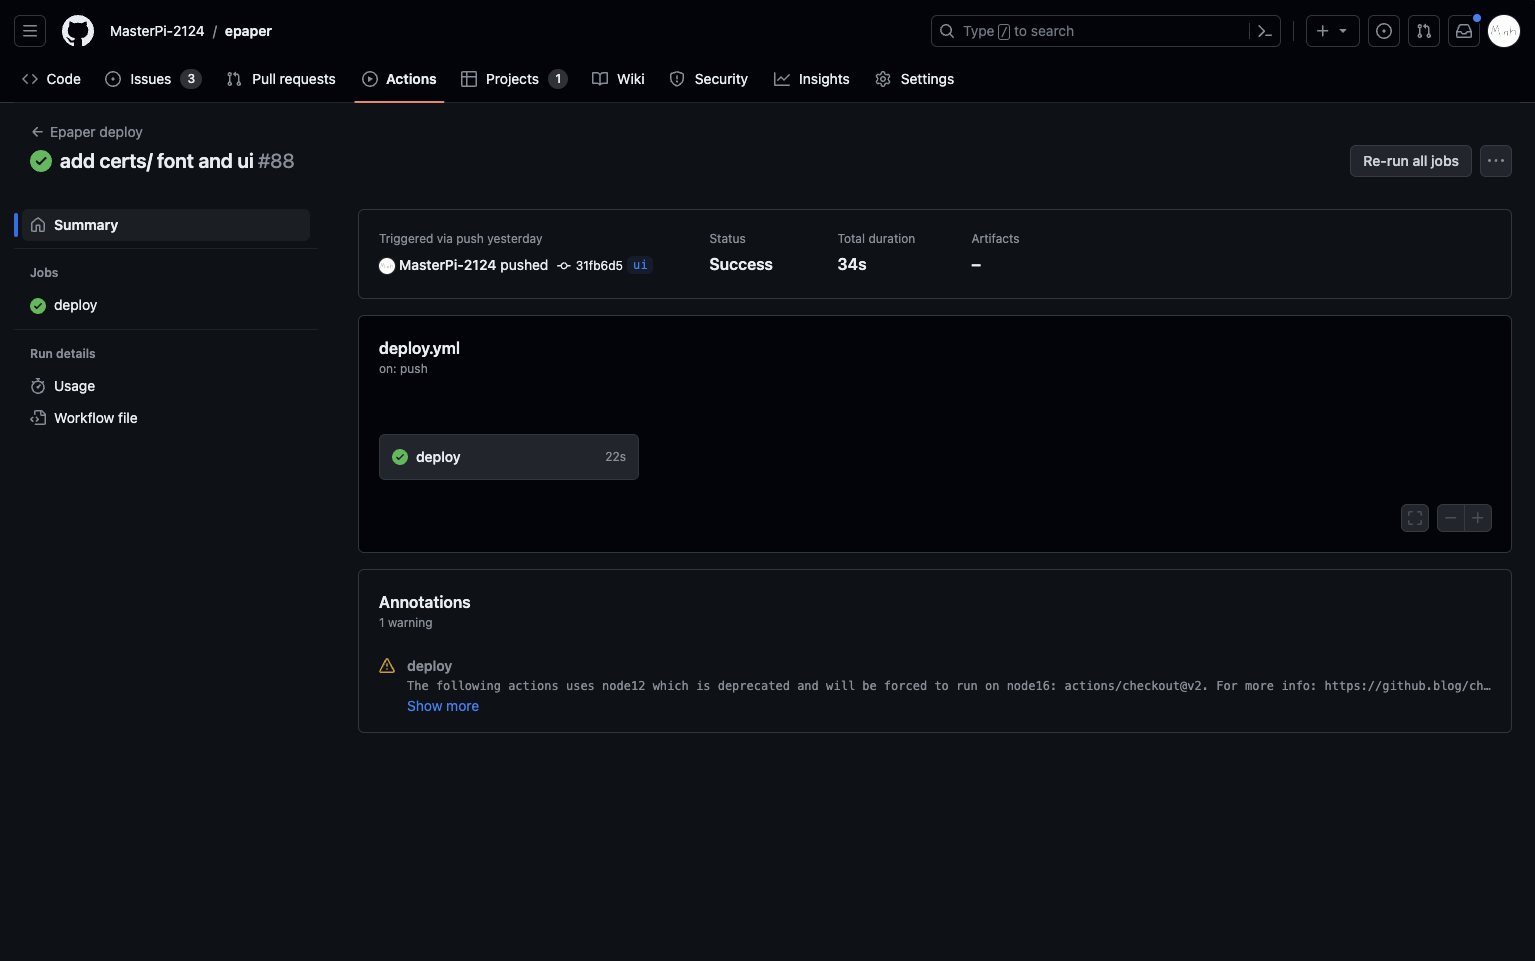
\includegraphics[width=0.9\linewidth]{doc//imgs/github_action.png}
    \caption{A successful GitHub deploy workflow}
    \label{fig:github-action}
\end{figure}

The project also releases stable firmware versions for EPD devices, which is listed on the GitHub "Releases"\footnote{Check out \url{https://github.com/MasterPi-2124/epaper/releases}} page. The releases are created from the stable \verb|main| branch, which is safe for developers to test the system. In each release, developers can download firmware for various microcontrollers (currently ESP32-C3 and ESP32-S2 variants), which are built and uploaded from \verb|ESP32 Build and Release| automated workflow in GitHub. The versions and release types are named in semantic format, with "Latest" meaning stable versions and "Pre-release" meaning stable beta versions with tested features or stable versions with minor updates.

\subsection{Servers}
The system uses two Hetzner dedicated servers to host the Rabbit MQTT broker and web services. Details of the servers and the tools used are shown in the table \ref{fig:table_tools} below.

\begin{table}[H]
    \newcolumntype{M}[1]{>{\centering\arraybackslash}m{#1}}
    \newcolumntype{L}[1]{>{\raggedright\arraybackslash}p{#1}}
    \renewcommand{\arraystretch}{3} % Adjust for row height
    \centering{}
    \fontsize{9pt}{8pt}\selectfont 
    \begin{tabular}{| m{2.5cm} | m{5.5cm} | m{5.5cm} |}
        \hline
                            & \textbf{API Server (web-server)}          & \textbf{MQTT Broker (laboratory)} \\ \hline
        IP address          & 65.108.79.164                             & 95.217.121.243                    \\ \hline
        Operating System    & Ubuntu 22.04.3 LTS x86\_64                & Ubuntu 22.04.3 LTS x86\_64        \\ \hline
        CPU                 & AMD Ryzen 5 3600 @ 3.600GHz               & AMD Ryzen 7 3700X @ 3.600GHz      \\ \hline
        RAM                 & 64GB                                      & 64GB                              \\ \hline
        Storage             & 1TB                                       & 2TB                               \\ \hline
        Purpose             & Management UI, API Server and proxy services         & MQTT broker                       \\ \hline
        Services used       & NginX, MongoDB, NextJS, NPM               & RabbitMQ                          \\ \hline
    \end{tabular}
    \caption{Detail of two Hetzner's dedicated servers}
    \label{fig:table_tools}
\end{table}

Both servers use RAID 1, creating a backup drive to store an exact copy of data on the main drive simultaneously. This clone mechanism ensures real-time data redundancy and high availability, thereby significantly enhancing data security and reducing the risk of data loss due to hardware failures, although the usable storage of the server is only half. It also offers improved read performance as the data can be read from multiple drives simultaneously.  

Services running in each server are configured as a system daemon (\verb|systemctl|), which is placed in \verb|/etc/systemd/system/| and \verb|/lib/systemd/system/|. Details of the services are listed in table \ref{fig:table_services} below.

\begin{table}[H]
    \newcolumntype{M}[1]{>{\centering\arraybackslash}m{#1}}
    \newcolumntype{L}[1]{>{\raggedright\arraybackslash}p{#1}}
    \renewcommand{\arraystretch}{3} % Adjust for row height
    \centering{}
    \fontsize{8pt}{8pt}\selectfont 
    \begin{tabular}{| m{4.2cm} | m{3.8cm} | m{3.4cm} | m{1.8cm} |}
        \hline
        \textbf{Services}               & \textbf{Name}             & \textbf{Location}             & \textbf{Server}   \\ \hline
        \verb|epaper.service|           & Epaper Front-end service  & \verb|/etc/systemd/system/|   & 65.108.79.164     \\ \hline
        \verb|epaper-backend.service|   & Epaper Back-end service   & \verb|/etc/systemd/system/|   & 65.108.79.164     \\ \hline
        \verb|rabbitmq-server.service|  & RabbitMQ broker service   & \verb|/lib/systemd/system/|   & 95.217.121.243    \\ \hline
        \verb|mongod.service|           & MongoDB Database service  & \verb|/lib/systemd/system/|   & 65.108.79.164     \\ \hline
        \verb|nginx.service|            & NginX daemon service      & \verb|/lib/systemd/system/|   & 65.108.79.164     \\ \hline
    \end{tabular}
    \caption{System services}
    \label{fig:table_services}
\end{table}

\subsection{EPD Devices}
The code is transferred and stored in ESP32-C3 Supermini flash memory using the PlatformIO plugin integrated into Visual Studio Code. The code takes about 1.5MB in total memory, most of which is stored in the non-volatile flash memory, meaning the code remains on the device even after it is powered off. The image of the ESP32-C3 Supermini and its ESP32-C3 microcontroller unit specs are listed in figure \ref{fig:esp32-c3} and table \ref{fig:table_c3specs} below.
The code is transferred and stored in ESP32-C3 Supermini flash memory using the PlatformIO plugin integrated into Visual Studio Code. The code takes about 1.5MB in total memory, most of which is stored in the non-volatile flash memory, meaning the code remains on the device even after it is powered off. The image of the ESP32-C3 Supermini and its ESP32-C3 microcontroller unit specs are listed in figure \ref{fig:esp32-c3} and table \ref{fig:table_c3specs} below.

\begin{figure}[H]
    \centering
    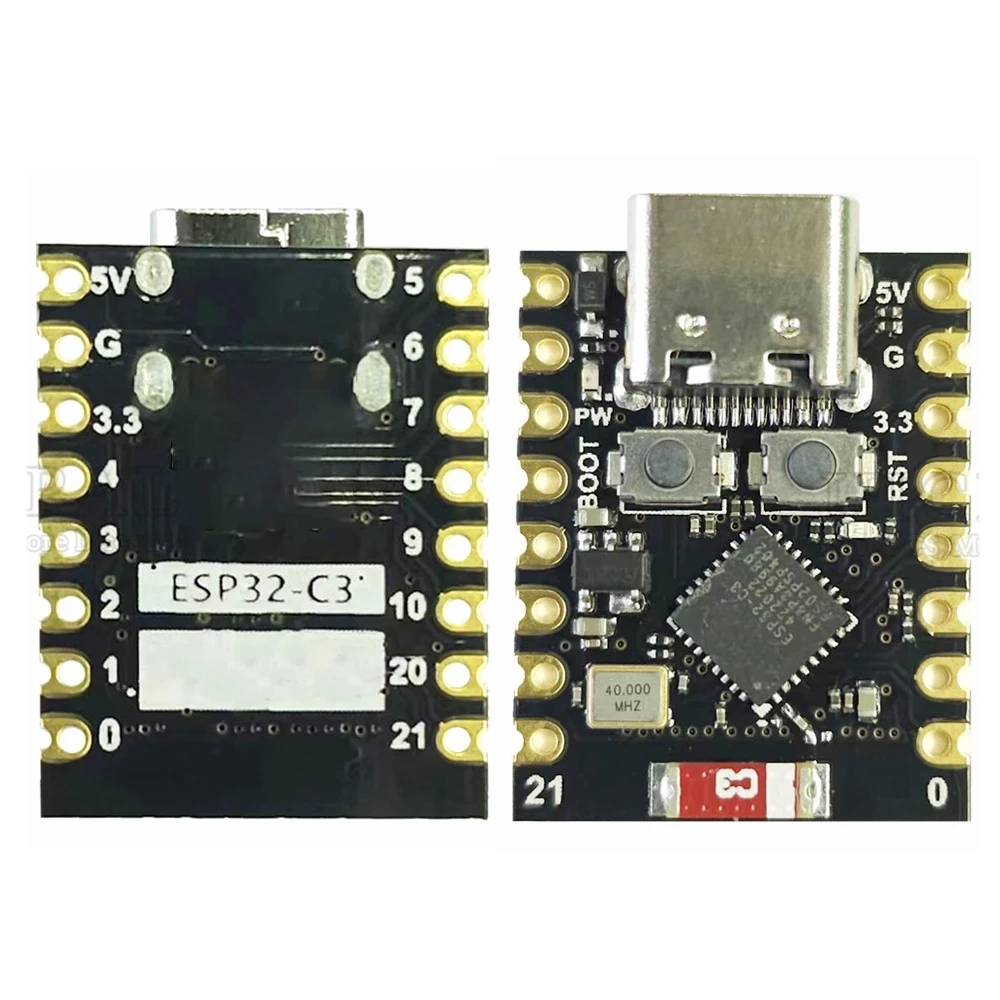
\includegraphics[width=0.75\linewidth]{doc//imgs/esp32-c3.png}
    \caption{Back and front image of ESP32-C3 Supermini}
    \label{fig:esp32-c3}
\end{figure}

\begin{table}[H]
    \newcolumntype{M}[1]{>{\centering\arraybackslash}m{#1}}
    \newcolumntype{L}[1]{>{\raggedright\arraybackslash}p{#1}}
    \renewcommand{\arraystretch}{3} % Adjust for row height
    \centering{}
    \fontsize{8pt}{8pt}\selectfont 
    \begin{tabular}{| m{4cm} | m{3.8cm} |}
        \hline
        \textbf{Attributes}     & \textbf{ESP32-C3}                                 \\ \hline
        Core                    & 32-bit RISC-V single-core (SoC)                   \\ \hline
        Maximum Clock Frequency & 160MHz                                            \\ \hline
        RAM size                & 400KB SRAM                                        \\ \hline
        Interfaces              & GPIO, I2C, I2S, SPI, UART                         \\ \hline
        Connectivities          & BLE 5.0, Wi-Fi (2.4GHz)                           \\ \hline
        Maximum transmit rate   & 150Mbps with Wi-Fi (2.4GHz), 2Mbps with BLE 5.0   \\ \hline
        Flash memory size       & 4MB                                               \\ \hline
        ROM                     & 384KB                                             \\ \hline
        Supply Voltage          & 3V - 3.6V                                         \\ \hline
    \end{tabular}
    \caption{ESP32-C3's specs}
    \label{fig:table_c3specs}
\end{table}

The e-paper display panel is connected and communicates to the board via SPI interfaces. Details of connected pins and their description are listed in table \ref{fig:table_spi} below.
\begin{table}[H]
    \newcolumntype{M}[1]{>{\centering\arraybackslash}m{#1}}
    \newcolumntype{L}[1]{>{\raggedright\arraybackslash}p{#1}}
    \renewcommand{\arraystretch}{3} % Adjust for row height
    \centering{}
    \fontsize{8pt}{8pt}\selectfont 
    \begin{tabular}{| m{1cm} | m{3cm} | m{6cm} |}
        \hline
        \textbf{Pin}    & \textbf{ESP32-C3 Supermini} & \textbf{Description}                          \\ \hline
        VCC             & 3V3	                      & Power input (3.3V)                            \\ \hline
        GND             & GND	                      & Ground                                        \\ \hline
        DIN	            & GPIO6                       & SPI MOSI pin, data input                      \\ \hline
        SCLK            & GPIO4                       & SPI CLK pin, clock signal input               \\ \hline
        CS              & GPIO7                       & Chip selection, low active                    \\ \hline
        DC              & GPIO1	                      & Data/command, low for commands, high for data \\ \hline
        RST             & GPIO2	                      & Reset, low active                             \\ \hline
        BUSY            & GPIO3	                      & Busy status output pin (means busy)           \\ \hline
    \end{tabular}
    \caption{SPI connection schematic}
    \label{fig:table_spi}
\end{table}

The device runs on battery, which can last 3 - 4 hours before recharging. In the scope of this project, this is still reasonable and acceptable as the product is still in the prototype stage and is not optimized for higher endurance in a real-life environment. 
\end{document}
